%definira klasu dokumenta 
\documentclass[12pt]{report} 

%prostor izmedu naredbi \documentclass i \begin{document} se zove uvod. U njemu se nalaze naredbe koje se odnose na cijeli dokument

%osnovni LaTex ne može riješiti sve probleme, pa se koriste različiti paketi koji olakšavaju izradu željenog dokumenta
\usepackage[croatian]{babel} 
\usepackage{amssymb}
\usepackage{amsmath}
\usepackage{txfonts}
\usepackage{mathdots}
\usepackage{titlesec}
\usepackage{array}
\usepackage{lastpage}
\usepackage{etoolbox}
\usepackage{tabularray}
\usepackage{color, colortbl}
\usepackage{adjustbox}
\usepackage{geometry}
\usepackage[classicReIm]{kpfonts}
\usepackage{hyperref}
\usepackage{fancyhdr}

\usepackage{float}
\usepackage{setspace}
\restylefloat{table}


\patchcmd{\chapter}{\thispagestyle{plain}}{\thispagestyle{fancy}}{}{} %redefiniranje stila stranice u paketu fancyhdr

%oblik naslova poglavlja
\titleformat{\chapter}{\normalfont\huge\bfseries}{\thechapter.}{20pt}{\Huge}
\titlespacing{\chapter}{0pt}{0pt}{40pt}


\linespread{1.3} %razmak između redaka

\geometry{a4paper, left=1in, top=1in,}  %oblik stranice

\hypersetup{ colorlinks, citecolor=black, filecolor=black, linkcolor=black,	urlcolor=black }   %izgled poveznice


%prored smanjen između redaka u nabrajanjima i popisima
\newenvironment{packed_enum}{
	\begin{enumerate}
		\setlength{\itemsep}{0pt}
		\setlength{\parskip}{0pt}
		\setlength{\parsep}{0pt}
	}{\end{enumerate}}

\newenvironment{packed_item}{
	\begin{itemize}
		\setlength{\itemsep}{0pt}
		\setlength{\parskip}{0pt}
		\setlength{\parsep}{0pt}
	}{\end{itemize}}




%boja za privatni i udaljeni kljuc u tablicama
\definecolor{LightBlue}{rgb}{0.9,0.9,1}
\definecolor{LightGreen}{rgb}{0.9,1,0.9}

%Promjena teksta za dugačke tablice
\DefTblrTemplate{contfoot-text}{normal}{Nastavljeno na idućoj stranici}
\SetTblrTemplate{contfoot-text}{normal}
\DefTblrTemplate{conthead-text}{normal}{(Nastavljeno)}
\SetTblrTemplate{conthead-text}{normal}
\DefTblrTemplate{middlehead,lasthead}{normal}{Nastavljeno od prethodne stranice}
\SetTblrTemplate{middlehead,lasthead}{normal}

%podesavanje zaglavlja i podnožja

\pagestyle{fancy}
\lhead{Programsko inženjerstvo}
\rhead{CookBooked}
\lfoot{Undercooked}
\cfoot{stranica \thepage/\pageref{LastPage}}
\rfoot{\today}
\renewcommand{\headrulewidth}{0.2pt}
\renewcommand{\footrulewidth}{0.2pt}


\begin{document} 
	
	
	
	\begin{titlepage}
		\begin{center}
			\vspace*{\stretch{1.0}} %u kombinaciji s ostalim \vspace naredbama definira razmak između redaka teksta
			\LARGE Programsko inženjerstvo\\
			\large Ak. god. 2023./2024.\\
			
			\vspace*{\stretch{3.0}}
			
			\huge CookBooked\\
			\Large Dokumentacija, Rev. \textit{1}\\
			
			\vspace*{\stretch{12.0}}
			\normalsize
			Grupa: Undercooked\\
			Voditelj: Eloise Habek\\
			
			
			\vspace*{\stretch{1.0}}
			Datum predaje: 17.11.2023.\\
	
			\vspace*{\stretch{4.0}}
			
			Nastavnik: Nikolina Frid\\
		
		\end{center}

	
	\end{titlepage}

	
	\tableofcontents


	\chapter{Dnevnik promjena dokumentacije}
		
		\textbf{\textit{Kontinuirano osvježavanje}}\\
				
		
		\begin{longtblr}[
				label=none
			]{
				width = \textwidth, 
				colspec={|X[2]|X[13]|X[3]|X[3]|}, 
				rowhead = 1
			}
			\hline
			\textbf{Rev.}	& \textbf{Opis promjene/dodatka} & \textbf{Autori} & \textbf{Datum}\\[3pt] \hline
			0.1 & Preuzet i popunjen predložak.	& Mateo Plavec & 19.10.2023. 		\\[3pt] \hline
			0.2	& Prva verzija \textit{Opisa projektnog zadatka} & Luka Grubišin & 27.10.2023.	\\[3pt] \hline 
			0.5 & Dodan \textit{Use Case} dijagram i jedan sekvencijski dijagram, funkcionalni i nefunkcionalni zahtjevi i dodatak A & * & 25.08.2013. \\[3pt] \hline 
			0.6 & Dodana struktura podataka i ER diagram baze podataka & Anabel Dautović & 08.11.2023. \\[3pt] \hline 
			0.8 & Povijest rada i trenutni status implementacije,\newline Zaključci i plan daljnjeg rada & * & 28.08.2013. \\[3pt] \hline 
			0.9 & Opisi obrazaca uporabe & * & 07.09.2013. \\[3pt] \hline 
			0.10 & Preveden uvod & * & 08.09.2013. \\[3pt] \hline 
			0.11 & Sekvencijski dijagrami & * & 09.09.2013. \\[3pt] \hline 
			0.12.1 & Započeo dijagrame razreda & * & 10.09.2013. \\[3pt] \hline 
			0.12.2 & Nastavak dijagrama razreda & * & 11.09.2013. \\[3pt] \hline 
			\textbf{1.0} & Verzija samo s bitnim dijelovima za 1. ciklus & * & 11.09.2013. \\[3pt] \hline 
			1.1 & Uređivanje teksta -- funkcionalni i nefunkcionalni zahtjevi & * \newline * & 14.09.2013. \\[3pt] \hline 
			1.2 & Manje izmjene:Timer - Brojilo vremena & * & 15.09.2013. \\[3pt] \hline 
			1.3 & Popravljeni dijagrami obrazaca uporabe & * & 15.09.2013. \\[3pt] \hline 
			1.5 & Generalna revizija strukture dokumenta & * & 19.09.2013. \\[3pt] \hline 
			1.5.1 & Manja revizija (dijagram razmještaja) & * & 20.09.2013. \\[3pt] \hline 
			\textbf{2.0} & Konačni tekst predloška dokumentacije  & * & 28.09.2013. \\[3pt] \hline 
			&  &  & \\[3pt] \hline	
		\end{longtblr}
	
	
		\textit{Moraju postojati glavne revizije dokumenata 1.0 i 2.0 na kraju prvog i drugog ciklusa. Između tih revizija mogu postojati manje revizije već prema tome kako se dokument bude nadopunjavao. Očekuje se da nakon svake značajnije promjene (dodatka, izmjene, uklanjanja dijelova teksta i popratnih grafičkih sadržaja) dokumenta se to zabilježi kao revizija. Npr., revizije unutar prvog ciklusa će imati oznake 0.1, 0.2, …, 0.9, 0.10, 0.11.. sve do konačne revizije prvog ciklusa 1.0. U drugom ciklusu se nastavlja s revizijama 1.1, 1.2, itd.}
	\chapter{Opis projektnog zadatka}
		
		% \textbf{\textit{dio 1. revizije}}\\
		
		% \textit{Na osnovi projektnog zadatka detaljno opisati korisničke zahtjeve. Što jasnije opisati cilj projektnog zadatka, razraditi problematiku zadatka, dodati nove aspekte problema i potencijalnih rješenja. Očekuje se minimalno 3, a poželjno 4-5 stranica opisa.	Teme koje treba dodatno razraditi u ovom poglavlju su:}
		% \begin{packed_item}
		% 	\item \textit{potencijalna korist ovog projekta}
		% 	\item \textit{postojeća slična rješenja (istražiti i ukratko opisati razlike u odnosu na zadani zadatak). Dodajte slike koja predočavaju slična rješenja.}
		% 	\item \textit{skup korisnika koji bi mogao biti zainteresiran za ostvareno rješenje.}
		% 	\item \textit{mogućnost prilagodbe rješenja }
		% 	\item \textit{opseg projektnog zadatka}
		% 	\item \textit{moguće nadogradnje projektnog zadatka}
		% \end{packed_item}
		
		% \textit{Za pomoć pogledati reference navedene u poglavlju „Popis literature“, a po potrebi konzultirati sadržaj na internetu koji nudi dobre smjernice u tom pogledu.}
		% \eject
		
		% \section{Primjeri u \LaTeX u}
		
		% \textit{Ovo potpoglavlje izbrisati.}\\
		% %Mislim da je ovo najbolje obrisati netom prije predaje ili kad se svi
		% %malo bolje upoznaju s LaTeXom, tu ima dosta korisnih primjera - Luka

		% U nastavku se nalaze različiti primjeri kako koristiti osnovne funkcionalnosti \LaTeX a koje su potrebne za izradu dokumentacije. Za dodatnu pomoć obratiti se asistentu na projektu ili potražiti upute na sljedećim web sjedištima:
		% \begin{itemize}
		% 	\item Upute za izradu diplomskog rada u \LaTeX u - \url{https://www.fer.unizg.hr/_download/repository/LaTeX-upute.pdf}
		% 	\item \LaTeX\ projekt - \url{https://www.latex-project.org/help/}
		% 	\item StackExchange za Tex - \url{https://tex.stackexchange.com/}\\
		
		% \end{itemize} 	


		
		% \noindent \underbar{podcrtani tekst}, \textbf{podebljani tekst}, 	\textit{nagnuti tekst}\\
		% \noindent \normalsize primjer \large primjer \Large primjer \LARGE {primjer} \huge {primjer} \Huge primjer \normalsize
				
		% \begin{packed_item}
			
		% 	\item  primjer
		% 	\item  primjer
		% 	\item  primjer
		% 	\item[] \begin{packed_enum}
		% 		\item primjer
		% 		\item[] \begin{packed_enum}
		% 			\item[1.a] primjer
		% 			\item[b] primjer
		% 		\end{packed_enum}
		% 		\item primjer
		% 	\end{packed_enum}
			
		% \end{packed_item}
		
		% \noindent primjer url-a: \url{https://www.fer.unizg.hr/predmet/proinz/projekt}
		
		% \noindent posebni znakovi: \# \$ \% \& \{ \} \_ 
		% $|$ $<$ $>$ 
		% \^{} 
		% \~{} 
		% $\backslash$ 
		
		
		% \begin{longtblr}[
		% 	label=none,
		% 	entry=none
		% 	]{
		% 		width = \textwidth,
		% 		colspec={|X[8,l]|X[8, l]|X[16, l]|}, 
		% 		rowhead = 1,
		% 	} %definicija širine tablice, širine stupaca, poravnanje i broja redaka naslova tablice
		% 	\hline \SetCell[c=3]{c}{\textbf{naslov unutar tablice}}	 \\ \hline[3pt]
		% 	\SetCell{LightGreen}IDKorisnik & INT	&  	Lorem ipsum dolor sit amet, consectetur adipiscing elit, sed do eiusmod  	\\ \hline
		% 	korisnickoIme	& VARCHAR &   	\\ \hline 
		% 	email & VARCHAR &   \\ \hline 
		% 	ime & VARCHAR	&  		\\ \hline 
		% 	\SetCell{LightBlue} primjer	& VARCHAR &   	\\ \hline 
		% \end{longtblr}
		

		% \begin{longtblr}[
		% 		caption = {Naslov s referencom izvan tablice},
		% 		entry = {Short Caption},
		% 	]{
		% 		width = \textwidth, 
		% 		colspec = {|X[8,l]|X[8,l]|X[16,l]|}, 
		% 		rowhead = 1,
		% 	}
		% 	\hline
		% 	\SetCell{LightGreen}IDKorisnik & INT	&  	Lorem ipsum dolor sit amet, consectetur adipiscing elit, sed do eiusmod  	\\ \hline
		% 	korisnickoIme	& VARCHAR &   	\\ \hline 
		% 	email & VARCHAR &   \\ \hline 
		% 	ime & VARCHAR	&  		\\ \hline 
		% 	\SetCell{LightBlue} primjer	& VARCHAR &   	\\ \hline 
		% \end{longtblr}
	


		
		
		% %unos slike
		% \begin{figure}[H]
		% 	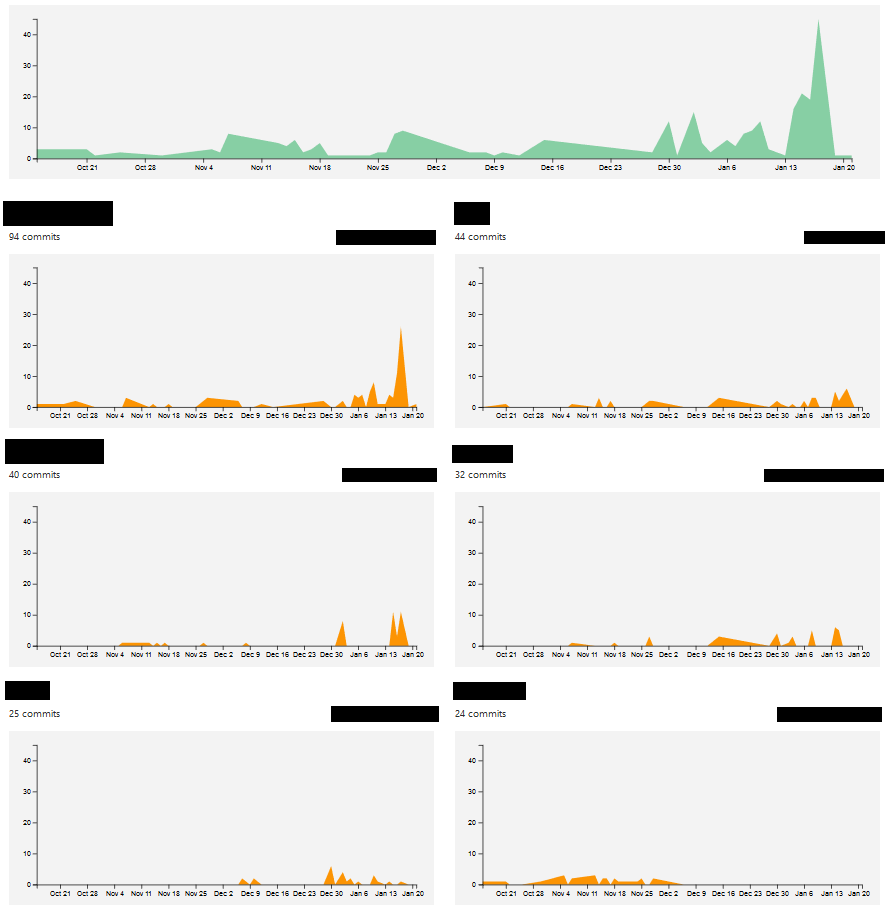
\includegraphics[scale=0.4]{slike/aktivnost.PNG} %veličina slike u odnosu na originalnu datoteku i pozicija slike
		% 	\centering
		% 	\caption{Primjer slike s potpisom}
		% 	\label{fig:promjene}
		% \end{figure}
		
		% \begin{figure}[H]
		% 	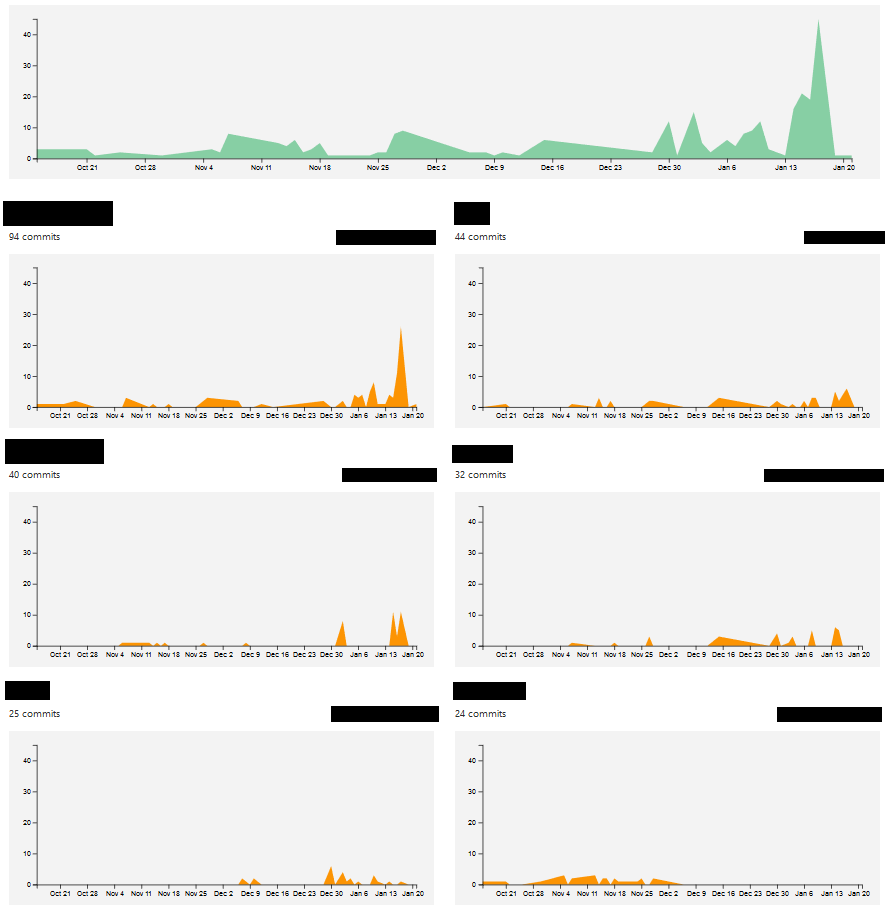
\includegraphics[width=\textwidth]{slike/aktivnost.PNG} %veličina u odnosu na širinu linije
		% 	\caption{Primjer slike s potpisom 2}
		% 	\label{fig:promjene2} %label mora biti drugaciji za svaku sliku
		% \end{figure}
		
		% Referenciranje slike \ref{fig:promjene2} u tekstu.
		
		% \eject
		
		\section{Uvod}
		\raggedright Cilj ovog projekta je razvoj web aplikacije za razmjenu recepata za pripremu kolača i diskusiju između korisnika i autora recepata koja bi ljudima omogućila jednostavno isprobavanje novih jela i poboljšanje svojih kulinarskih sposobnosti.
		\section{Postojeća rješenja i njihovi problemi}
		Postoje brojna popularna slična rješenja, no uglavnom pate od loše preglednosti zbog previše prevelikih slika, puno praznog prostora i velike količine popratnog teksta koji nema veze sa sastojcima ili pripremom kao što je prikazano na slikama \ref{fig:primjer1} i \ref{fig:primjer2} u nastavku. 
		\begin{figure}[H]
			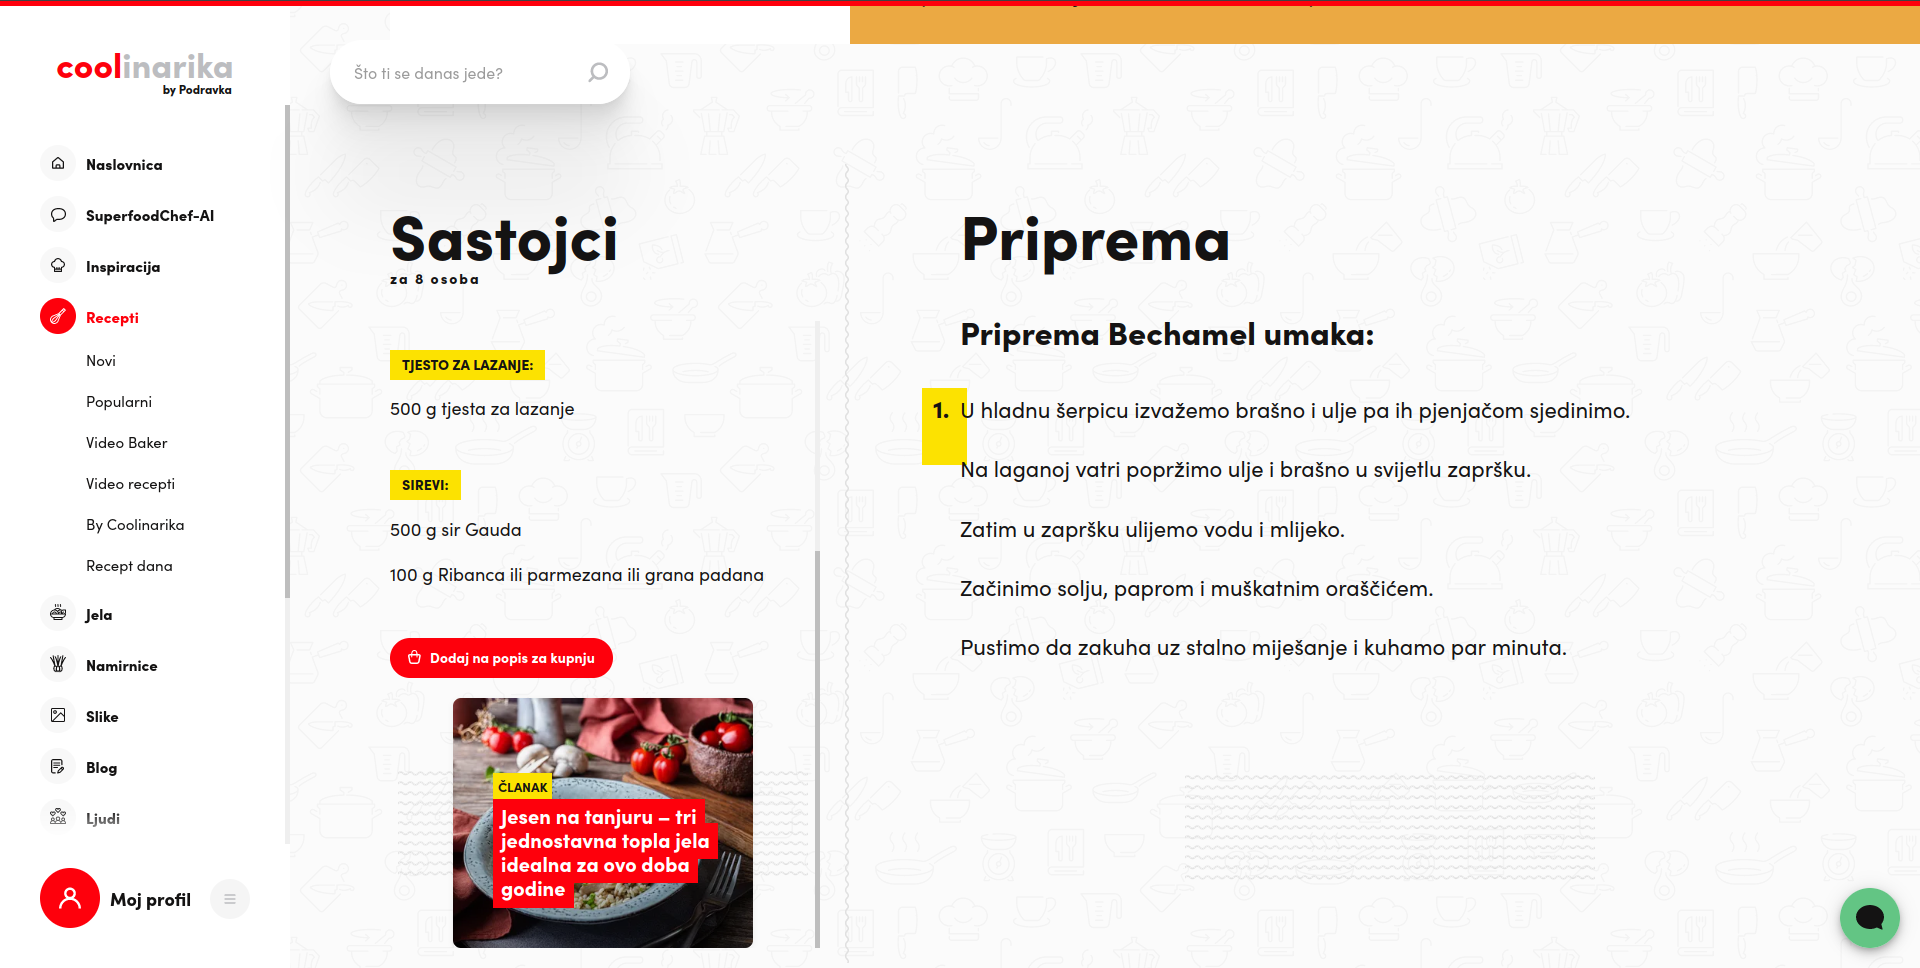
\includegraphics[scale=0.24]{slike/primjer_coolinarika.png}
			\centering
			\caption{Coolinarika - Prevelika slova, puno neiskorištenog prostora}
			\label{fig:primjer1}
		\end{figure}
		\begin{figure}[H]
			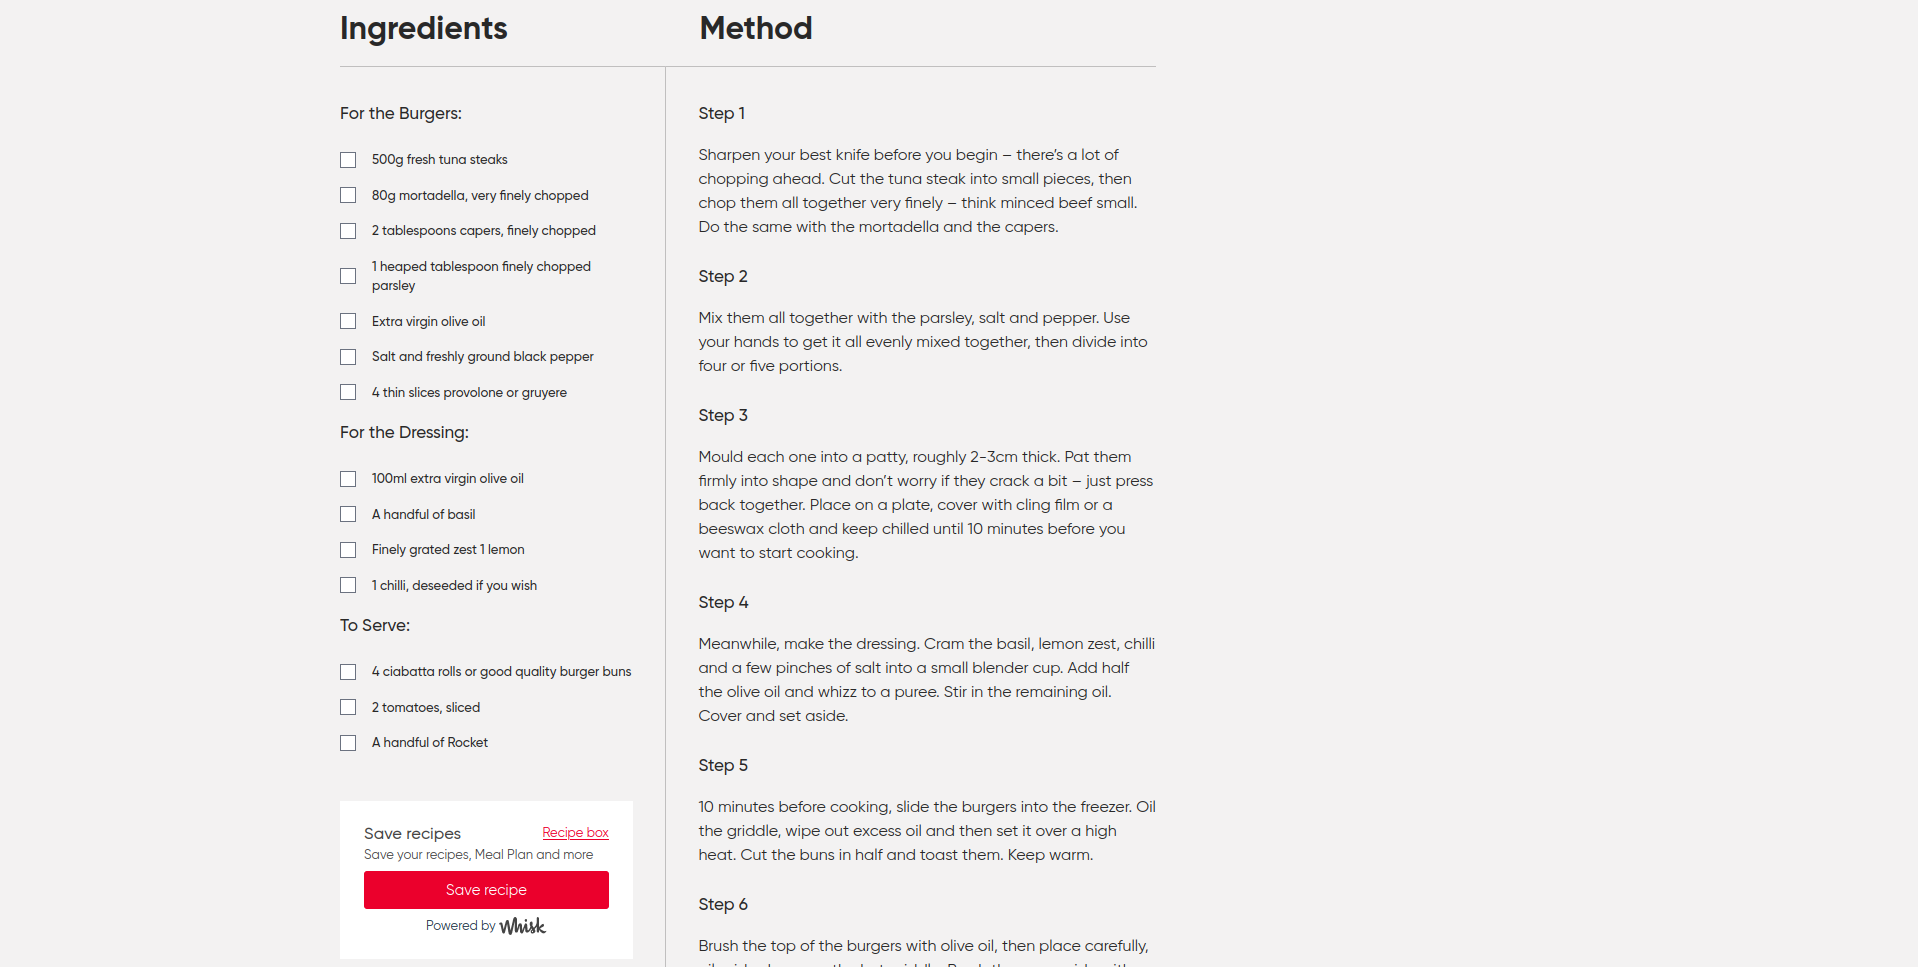
\includegraphics[scale=0.24]{slike/primjer_foodnetwork.png}
			\centering
			\caption{Foodnetwork - Preglednije, ali i dalje puno praznog prostora}
			\label{fig:primjer2}
		\end{figure}
		Recepti bi trebali sadržavati samo informacije važne za pripremu i možda jednu ili dvije uvodne rečenice. Većina recepata trebala bi stati na jednu stranicu kako bi bili pregledniji, ali i kako bi ih se lako moglo ispisati na papir. Ovakav izgled stranice nije uvijek jednostavno ostvariti, ali bi trebao uvelike poboljšati iskustvo korištenja.
		\section{Osnovne mogućnosti stranice}
		Glavna mogućnost stranice je naravno, prikazivanje sastojaka i uputa za pripremu, ali osim njih, recepti sadrže i brojne druge informacije koje olakšavaju pripremu i traženje sličnih recepata kao što su:
		\begin{packed_item}
			\item kategorija jela
			\item vrsta kuhinje
			\item neuobičajeni sastojci
			\item alergeni
			\item vrijeme pripreme
			\item broj porcija
			\item ostale oznake
		\end{packed_item}
		Stranica razlikuje dvije vrste korisnika: goste, odnosno neregistrirane korisnike, i registrirane korisnike. Neregistrirani korisnici mogu pristupiti samo osnovnim funkcionalnostima stranice. Imaju potpuni pristup svim receptima te mogu pretraživati recepte po prije navedenim oznakama ili po njihovom nazivu. Isto tako mogu uz neka ograničenja pregledavati profile registriranih korisnika. Ovo će većini korisnika koji samo povremeno traže nove recepte ili inspiraciju vjerojatno biti dovoljno, a oni koji žele pristupiti naprednijim pogodnostima koje stranica nudi moraju se registrirati.
		\linebreak
		Postupak registracije vrlo je jednostavan. Potrebno je samo navesti sljedeće podatke kako bi korisnik stvorio novi profil:
		\begin{packed_item}
			\item korisnično ime
			\item adresu elektroničke pošte
			\item lozinku
		\end{packed_item}
		
		\section{Napredne mogućnosti stranice}
		Nakon što se korisnik registrira i prijavi, otvaraju mu se brojne dodatne mogućnosti stranice. Najvažnija i najzanimljivija je naravno mogućnost objave vlastitih recepata. Kako bi korisnik objavio recept, mora navesti naziv recepta, sastojke, postupak pripreme i ukupno trajanje pripreme. Ostali podatci nisu neophodni, ali ih je korisno navesti kako bi zainteresirani korisnici mogli brže i jednostavnije naći recepte koji odgovaraju njihovim željama i potrebama.
		\linebreak
		\linebreak
		Svaki registrirani korisnik također može označavati i spremati recepte na svoj osobni profil kako bi mu u budućnosti bili lako dostupni, a isto tako mogu zapratiti druge autore kako bi bili automatski obaviješteni kada netko od njihovih najdražih autora objavi novi recept.
		Objavljeni recepti, pratitelji i osobe koje prate korisnika javno su vidljivi na profilu svakog korisnika.
		\section{Komunikacija među korisnicima}
		Osim što mogu ostavljati komentare na receptima i tako komunicirati s autorom i drugim korisnicima, registrirani korisnici također imaju mogućnost izravnog kontaktiranja autora recepata ako trebaju dodatna pojašnjenja ili žele uputiti svoje pohvale (ili kritike) autoru. Aplikacija omogućava jednostavnu razmjenu poruka između korisnika, ali isto tako, autor može navesti i druge načine na koje ga se može kontaktirati, kao što su elektronička pošta ili broj telefona. Također može navesti i vremenske periode u kojima je dostupan.
		\section{Administracija}
		Osim gostiju i registriranih korisnika, važan čimbenik u radu stranice su i administratori. Administratori imaju vlastite korisničke profile, kao i obični registrirani korisnici, ali imaju dodatne ovlasti koje im omogućavaju upravljanje stranicom.
		\linebreak
		Ovlasti administratora uključuju:
		\begin{packed_item}
			\item upravljanje korisnicima
			\item[] \begin{packed_item}
					\item brisanje korisnika
					\item uređivanje korisničkih profila
					\item dodavanje korisnika
					\end{packed_item}
			\item upravljanje receptima
			\item[] \begin{packed_item}
					\item brisanje recepata
					\item uređivanje recepata
					\item mijenjanje oznaka recepata
					\end{packed_item}
		\end{packed_item}
		
	
	\chapter{Specifikacija programske potpore}
		
	\section{Funkcionalni zahtjevi}
			
			% \textbf{\textit{dio 1. revizije}}\\
			
			% \textit{Navesti \textbf{dionike} koji imaju \textbf{interes u ovom sustavu} ili  \textbf{su nositelji odgovornosti}. To su prije svega korisnici, ali i administratori sustava, naručitelji, razvojni tim.}\\
				
			% \textit{Navesti \textbf{aktore} koji izravno \textbf{koriste} ili \textbf{komuniciraju sa sustavom}. Oni mogu imati inicijatorsku ulogu, tj. započinju određene procese u sustavu ili samo sudioničku ulogu, tj. obavljaju određeni posao. Za svakog aktora navesti funkcionalne zahtjeve koji se na njega odnose.}\\
			
			
			\noindent \textbf{Dionici:}
			
			\begin{packed_enum}
				
				\item Nikolina Frid
				\item Andrija Gorup 
				\item Razvojni tim
				\item Korisnici
				\item Administrator
				
			\end{packed_enum}
			
			\noindent \textbf{Aktori i njihovi funkcionalni zahtjevi:}
			
			
			\begin{packed_enum}

				\item  \underbar{korisnik (inicijator) može:}
				
				\begin{packed_enum}
					
					\item pretražiti recept po značajkama
					\item pregledati recept
					\item osvježiti broj porcija, čime će se ažurirati mjerice sastojaka u skladu s navedenim brojem porcija
					\item otvoriti profile registriranih korisnika koji su postavili recept
					
				\end{packed_enum}

				\item  \underbar{Neregistrirani korisnik (inicijator) može:}
				
				\begin{packed_enum}

					\item sve što i korisnik (specijalizacija korisnika)
					\item otvoriti novi korisnički račun za koji je potrebno unjeti korisničko ime koje nije već zauzeto, adresu elektroničke pošte i lozinku računa
					
				\end{packed_enum}

				\item  \underbar{Registrirani korisnik (inicijator) može:}
				
				\begin{packed_enum}
					
					\item sve što i korisnik (specijalizacija korisnika)
					\item ažurirati profil, podaci koje je moguće ažurirati su email, broj telefona i vremenski period u kojima je korisnik dostupan
					\item objaviti recept s obaveznim navođenjem naziva recepta, sastojaka, postupka pripreme i ukupnog trajanja pripreme, mogućnost navođenja dodatnih karakteristika poput oznaka tipa jela i dodavanja slika i videozapisa
					\item ažuriranje već objavljenih recepata
					\item ocijeniti objavu
					\item spremiti recept kako bi im mogli lakše pristupiti kasnije
					\item zapratiti drugog autora (registriranog korisnika), korisnik će dobiti obavijest kada autor objavi novi recept
					\item pregledati vlastiti profil
					\item dodavanje nove oznake poput kategorije ili vrste kuhinje
					\item brisati recepte sa svojeg profila
					\item pisanje komentara na recepte drugih korisnika
					\item slanje poruka u privatnom chatu
					\item pregled poruka privatnih chatova
					
				\end{packed_enum}

				\item  \underbar{Administrator (inicijator) može:}
				\begin{packed_enum}

					\item sve što i korisnik (specijalizacija korisnika)
					\item brisanje korisničkog profila
					\item brisanje recepata
					\item dodati novog administratora
					\item pregled mogućnosti administratora
					\item pristupiti statistikama (npr. najpopularniji recept po broju profila koji su ga spremili, najaktivniji profil s najviše recepata, najpopularniji profil s najčešće spremljenim receptima)
					\item brisanje komentara koji nisu u skladu s pravilima ophođenja na platformi

				\end{packed_enum}
			
				\item  \underbar{Baza podataka (sudionik) može:}
				
				\begin{packed_enum}
					
					\item pohranjuje sve podatke o korisnicima i njihovim ovlastima
					\item pohranjuje sve podatke o receptima
					\item pohranjuje informacije o odnosima među korisnika i recepata
					
				\end{packed_enum}
			\end{packed_enum}
			
			\eject 
			
			
				
			\subsection{Obrasci uporabe}
					
					%Općenita napomena za UC - u .txt skici se kao sudionik često navodi back-end
					%Budući da nije naveden u aktorima, umjesto toga piše baza podataka
					\noindent \underbar{\textbf{UC1 - Pregled recepta}}
					\begin{packed_item}
						
						\item \textbf{Glavni sudionik: }Korisnik
						\item \textbf{Cilj: }Pregledati objavljene recepte
						\item \textbf{Sudionici: }Baza podataka
						\item \textbf{Preduvjet: }-
						\item \textbf{Opis osnovnog tijeka:}
						
						\item[] \begin{packed_enum}
								\item Korisnik odabire recept koji se prikaže
								\end{packed_enum}
					\end{packed_item}
					
					\noindent \underbar{\textbf{UC2 - Pretraživanje recepata}}
					\begin{packed_item}
						
						\item \textbf{Glavni sudionik: }Korisnik
						\item \textbf{Cilj: }Prikazati recepte u skladu s podatcima unesenim u tražilicu
						\item \textbf{Sudionici: }Baza podataka
						\item \textbf{Preduvjet: }-
						\item \textbf{Opis osnovnog tijeka:}
						
						\item[] \begin{packed_enum}
							\item Korisnik odabire pretraživanje recepata
							\item Upisuje ključnu riječ (kategorija, vrsta kuhinje, specifični sastojci)
							\item Baza podataka vraća recepte koji odgovaraju parametrima pretrage
							\item Dobiveni recepti prikazuju se u aplikaciji
						\end{packed_enum}
						\item \textbf{Opis mogućih odstupanja:}
						\item[] \begin{packed_enum}
							\item[3.a] U bazi podataka ne nalazi se niti jedan recept koji odgovara unesenim parametrima
							\begin{packed_enum}
								\item[1.] Sustav korisniku prikazuje poruku da trenutno nema recepata koji odgovaraju njegovom unosu
							\end{packed_enum}
						\end{packed_enum}
					\end{packed_item}
					
					\noindent \underbar{\textbf{UC3 - Registriranje novog korisnika}}
					\begin{packed_item}
						
						\item \textbf{Glavni sudionik: }Neregistrirani korisnik
						\item \textbf{Cilj: }Stvaranje novog korisničkog računa
						\item \textbf{Sudionici: }Baza podataka
						\item \textbf{Preduvjet: }-
						\item \textbf{Opis osnovnog tijeka:}
						%Ovo će možda trebati mijenjati u budućnosti kada budemo radili implementaciju
						\item[] \begin{packed_enum}
							\item Neregistrirani korisnik odabire opciju za registraciju
							\item Unosi potrebne podatke (korisničko ime, adresu elektroničke pošte i lozinku)
							\item Baza podataka provjerava jesu li korisničko ime ili e-mail adresa već zauzeti
							\item Ako su korisničko ime i e-mail adresa slobodni, novog registriranog korisnika se upisuje u bazu
							\item Učitava se naslovna stranica
						\end{packed_enum}
						\item \textbf{Opis mogućih odstupanja:}
						\item[] \begin{packed_enum}
							\item[3.a] Korisničko ime ili adresa elektroničke pošte već su zauzeti
							\begin{packed_enum}
								\item[1.] Korisnik dobiva poruku da su korisničko ime ili e-mail adresa već korišteni
								\item[2.] Korisnika se traži ponovni upis podataka
							\end{packed_enum}
						\end{packed_enum}
					\end{packed_item}
					
					\noindent \underbar{\textbf{UC4 - Prikazivanje tuđeg korisničkog profila}}
					\begin{packed_item}
						
						\item \textbf{Glavni sudionik: }Korisnik
						\item \textbf{Cilj: }Pregled profila drugog registriranog korisnika
						\item \textbf{Sudionici: }Baza podataka
						\item \textbf{Preduvjet: }-
						\item \textbf{Opis osnovnog tijeka:}
						
						\item[] \begin{packed_enum}
							\item Korisnik odabire ikonu autora neke objave
							\item Korisniku se prikazuje profil autora
						\end{packed_enum}
						\item \textbf{Opis mogućih odstupanja:}
						\item[] \begin{packed_enum}
							\item[1.a] Korisnik koristi tražilicu kako bi našao profil koji želi pregledati
							%Što ako koristi tražilicu i nema ničega? Je li to odstupanje na odstupanje? Pitati demosa/asistenta?
							\item[] \begin{packed_enum}
								\item[1.] Korisnik odabire jedan od profila dobivenih pretragom
								\item[2.] Korisniku se prikazuje odabrani profil
							\end{packed_enum}
							\item[2.a] Korisnik pregledava profil koji prati
							\item[] \begin{packed_enum}
								\item[1.] Korisnik otvara vlastiti profil
								\item[2.] Odabire opciju za prikaz profila koje prati
								\item[3.] Korisnik odabire jedan od navedenih profila
								\item[4.] Prikazuje se odabrani profil
							\end{packed_enum}
						\end{packed_enum}
					\end{packed_item}

					\noindent \underbar{\textbf{UC5 - Ažuriranje broj porcija}}
					\begin{packed_item}
						
						\item \textbf{Glavni sudionik: }Korisnik
						\item \textbf{Cilj: }Prikazati potrebne sastojke recepta u skladu s potrebnim porcijama jela
						\item \textbf{Sudionici: }Baza podataka
						\item \textbf{Preduvjet: }UC1 (Pregled recepta)
						\item \textbf{Opis osnovnog tijeka:}
						
						\item[] \begin{packed_enum}
							\item Korisnik na prikazanom receptu stiskanjem tipki (+/-) ažurira broj porcija
							\item Prikaz recepta se ažurira s obzirom na broj porcija
						\end{packed_enum}
					\end{packed_item}

					\noindent \underbar{\textbf{UC6 - Prijava}}
					\begin{packed_item}
						
						\item \textbf{Glavni sudionik: }Registrirani korisnik, Administrator
						\item \textbf{Cilj: }Dobivanje pristupa mogućnostima registriranog korisnika
						\item \textbf{Sudionici: }Baza podataka
						\item \textbf{Preduvjet: }UC3 (Registracija)
						\item \textbf{Opis osnovnog tijeka:}
						
						\item[] \begin{packed_enum}
							\item Registrirani korisnik na naslovnoj stranici odabire opciju za prijavu
							\item Korisnik unosi potrebne podatke (e-mail adresu i lozinku)
							\item Baza podataka provjerava je li korisnik registriran
							\item Baza podataka provjerava je li lozinka ispravna
							\item Učitava se naslovna stranica
						\end{packed_enum}
						\item \textbf{Opis mogućih odstupanja:}
						\item[] \begin{packed_enum}
							\item[3.a] Korisnik nije registriran
							\begin{packed_enum}
								\item[1.] Korisnik dobiva poruku da nije registriran
								\item[2.] Korisnika se preusmjerava na obrazac za registraciju
							\end{packed_enum}
							\item[4.a] Lozinka nije ispravna
							\begin{packed_enum}
								\item[1.] Korisnika se traži da upiše ispravnu lozinku
							\end{packed_enum}
						\end{packed_enum}
					\end{packed_item}
					
					\noindent \underbar{\textbf{UC7 - Objava recepta}}
					\begin{packed_item}
						
						\item \textbf{Glavni sudionik: }Registrirani korisnik
						\item \textbf{Cilj: }Objava novog recepta
						\item \textbf{Sudionici: }Baza podataka
						\item \textbf{Preduvjet: }UC6 (Prijava)
						\item \textbf{Opis osnovnog tijeka:}
						
						\item[] \begin{packed_enum}
							\item Korisnik odabire opciju za novu objavu
							\item Korisnik unosi naslov recepta, sastojke, upute za pripremu i vrijeme pripreme te po izboru dodaje i oznake kategorija, slike i videozapise
							\item Baza podataka zapisuje novi recept i moguće nove oznake unesene
							\item Svi pratitelji autora dobivaju obavijest o novom receptu
						\end{packed_enum}
					\end{packed_item}
					
					\noindent \underbar{\textbf{UC8 - Uređivanje objave}}
					\begin{packed_item}
						
						\item \textbf{Glavni sudionik: }Registrirani korisnik
						\item \textbf{Cilj: }Urediti prethodno objavljeni recept
						\item \textbf{Sudionici: }Baza podataka
						\item \textbf{Preduvjet: }UC7 (Objava recepta)
						\item \textbf{Opis osnovnog tijeka:}
						
						\item[] \begin{packed_enum}
							\item Korisnik odabire pregled vlastitog profila
							\item Korisnik odabire objavu koju želi urediti
							\item Odabire opciju za uređivanje
							\item Korisnik uređuje sadržaj recepta
							\item Po završetku odabire opciju za kraj uređivanja
							\item Baza podataka ažurira recept i dodaje moguće nove oznake
						\end{packed_enum}
					\end{packed_item}
					
					\noindent \underbar{\textbf{UC9 - Brisanje objave}}
					\begin{packed_item}
						
						\item \textbf{Glavni sudionik: }Registrirani korisnik
						\item \textbf{Cilj: }Brisanje prethodno objavljenog recepta
						\item \textbf{Sudionici: }Baza podataka
						\item \textbf{Preduvjet: }UC7 (Objava recepta)
						\item \textbf{Opis osnovnog tijeka:}
						
						\item[] \begin{packed_enum}
							\item Korisnik odabire pregled vlastitog profila
							\item Korisnik odabire objavu koju želi obrisati
							\item Korisnik odabire opciju za brisanje
							\item Baza podataka briše odabrani recept
						\end{packed_enum}
					\end{packed_item}
					
					
					
					\noindent \underbar{\textbf{UC10 - Slanje poruke drugom registriranom korisniku}}
					\begin{packed_item}
						
						\item \textbf{Glavni sudionik: }Registrirani korisnik
						\item \textbf{Cilj: }Komunikacija među korisnicima putem poruka
						\item \textbf{Sudionici: }Baza podataka
						\item \textbf{Preduvjet: } UC4 (Prikazivanje tuđeg profila)
						\item \textbf{Opis osnovnog tijeka:}
						
						\item[] \begin{packed_enum}
							\item Korisnik odabire opciju za slanje poruke
							\item Otvara se polje za pisanje poruke
							\item Kada napiše poruku, korisnik odabire opciju za slanje
							\item Poruka se upisuje u bazu podataka u inbox primatelja
						\end{packed_enum}
					\end{packed_item}
					
					\noindent \underbar{\textbf{UC11 - Zaprati korisnika}}
					\begin{packed_item}
						
						\item \textbf{Glavni sudionik: }Registrirani korisnik
						\item \textbf{Cilj: }Praćenje drugog korisnika kako bi dobio obavijesti o novim objavama
						\item \textbf{Sudionici: }Baza podataka
						\item \textbf{Preduvjet: }UC4 (Prikazivanje tuđeg profila)
						\item \textbf{Opis osnovnog tijeka:}
						
						\item[] \begin{packed_enum}
							\item Korisnik odabire opciju za praćenje
							\item Baza podataka ažurira popis praćenih korisnika
						\end{packed_enum}
					\end{packed_item}
					
					\noindent \underbar{\textbf{UC12 - Pozovi korisnika na video poziv}}
					\begin{packed_item}
						%Možda ne bi bilo loše ovo razraditi čak i ako nećemo implementirati
						%Imati ćemo nešto za napisati u poglavlju 6 - Zaključak i budući rad
						%"Potrebno je točno popisati funkcionalnosti koje nisu implementirane u ostvarenoj aplikaciji"
						\item \textbf{Glavni sudionik: }Registrirani korisnik (Pozivatelj)
						\item \textbf{Cilj: }Uspostava komunikacije između dva korisnika putem videopoziva
						\item \textbf{Sudionici: }Registrirani korisnik (Korisnik kojeg se zove)
						\item \textbf{Preduvjet: }UC4 (Prikazivanje tuđeg profila)
						\item \textbf{Opis osnovnog tijeka:}
						
						\item[] \begin{packed_enum}
							\item Pozivatelj odabire opciju za pokretanje videopoziva
							\item Korisnik kojeg se zove dobiva obavijest o pozivu
							\item Korisnik kojeg se zove prihvaća poziv
							\item Korisnici razgovaraju
							\item Jedan od korisnika prekida poziv po završetku razgovora
						\end{packed_enum}
						\item \textbf{Opis mogućih odstupanja:}
						\item[] \begin{packed_enum}
							\item[3.a] Korisnik kojeg se zove odbija pozivi ili se ne javlja
							\begin{packed_enum}
								\item[1.] Pozivatelj dobiva poruku da je korisnik kojeg zove nedostupan
							\end{packed_enum}
						\end{packed_enum}
					\end{packed_item}
					
					\noindent \underbar{\textbf{UC13 - Pregled inboxa}}
					\begin{packed_item}
						
						\item \textbf{Glavni sudionik: }Registrirani korisnik
						\item \textbf{Cilj: }Pregled svih poruka i obavijesti
						\item \textbf{Sudionici: }Baza podataka
						\item \textbf{Preduvjet: }UC6 (Prijava)
						\item \textbf{Opis osnovnog tijeka:}
						
						\item[] \begin{packed_enum}
							\item Korisnik odabire opciju za pregled inboxa
							\item Otvara se stranica s popisom svih poruka i obavijesti
						\end{packed_enum}
					\end{packed_item}
					
					\noindent \underbar{\textbf{UC14 - Odgovaranje na poruku}}
					\begin{packed_item}
						
						\item \textbf{Glavni sudionik: }Registrirani korisnik
						\item \textbf{Cilj: }Poslati odgovor na dobivenu poruku
						\item \textbf{Sudionici: }Baza podataka
						\item \textbf{Preduvjet: }UC13 (Otvaranje inboxa)
						\item \textbf{Opis osnovnog tijeka:}
						
						\item[] \begin{packed_enum}
							\item Korisnik odabire opciju za otvaranje inboxa
							\item Korisnik odabire poruku na koju želi odgovoriti
							\item Odabire opciju za odgovor
							\item Otvara se polje za sastavljanje poruke
							\item Korisnik piše odgovor
							\item Kada je gotov, odabire opciju za slanje
							\item Poruka se upisuje u bazu podataka u inbox primatelja
						\end{packed_enum}
					\end{packed_item}
					
					%Ovo možda razdvojiti na dva UC-a ili ostaviti samo jednu od opcija
					%Pričali smo o ovome ali ne sijećam se koji je na kraju bio zaključak
					\noindent \underbar{\textbf{UC15 - Ocijeni objavu}}
					\begin{packed_item}
						
						\item \textbf{Glavni sudionik: }Registrirani korisnik
						\item \textbf{Cilj: }Ocijeniti recept s ocjenom od 1 do 5
						\item \textbf{Sudionici: }Baza podataka
						\item \textbf{Preduvjet: }UC6 (Prijava)
						\item \textbf{Opis osnovnog tijeka:}
						
						\item[] \begin{packed_enum}
							\item Korisnik otvara recept koji želi ocijeniti
							\item Korisnik odabire ocjenu koju želi dati
							\item U bazi podataka se ažurira ocjena
						\end{packed_enum}
					\end{packed_item}
					
					\noindent \underbar{\textbf{UC16 - Spremi recept}}
					\begin{packed_item}
						
						\item \textbf{Glavni sudionik: }Registrirani korisnik
						\item \textbf{Cilj: }Spremiti recept kako bi ga se kasnije moglo lakše opet pronaći
						\item \textbf{Sudionici: } Baza podataka
						\item \textbf{Preduvjet: } UC6 (Prijava)
						\item \textbf{Opis osnovnog tijeka:}
						
						\item[] \begin{packed_enum}
							\item Korisnik otvara recept koji želi spremiti
							\item Odabire opciju za spremanje recepta
							\item U bazi podataka se ažurira relacija spremanja u odnosu na korisnika i recepta
						\end{packed_enum}
					\end{packed_item}
										
					\noindent \underbar{\textbf{UC17 - Komentiraj objavljeni recept}}
					\begin{packed_item}
						
						\item \textbf{Glavni sudionik: } Registrirani korisnik
						\item \textbf{Cilj: }Ostaviti komentar na nekoj objavi
						\item \textbf{Sudionici: }Baza podataka
						\item \textbf{Preduvjet: }UC6 (Prijava)
						\item \textbf{Opis osnovnog tijeka:}
						
						\item[] \begin{packed_enum}
							\item Korisnik otvara objavljeni recept
							\item Korisnik otvara komentare na objavi
							\item Korisnik odabire opciju za pisanje komentara
							\item Otvara se polje za pisanje komentara
							\item Korisnik piše komentar i zatim odabire opciju za objavu
							\item Komentar se zapisuje u bazu podataka
						\end{packed_enum}
							%Tek mi je ovdje palo na pamet, ali ista stvar vrijedi i za druge UC-ove
							%Treba li dodati opciju za odustajanje od pisanja komentara?
							%To bi onda vjerojatno bilo odstupanje, ali vjerojatno cijela ideja predstavlja previše nepotrebnog filozofiranja
					\end{packed_item}
										
					\noindent \underbar{\textbf{UC18 - Pregled vlastitog profila}}
					\begin{packed_item}
						
						\item \textbf{Glavni sudionik: }Registrirani korisnik
						\item \textbf{Cilj: }Pregledati stanje vlastitog korisničkog profila
						\item \textbf{Sudionici: }Baza podataka
						\item \textbf{Preduvjet: }UC6 (Prijava)
						\item \textbf{Opis osnovnog tijeka:}
						
						\item[] \begin{packed_enum}
							\item Korisnik na početnoj stranici odabire svoju ikonu
							\item Otvara se stranica na kojoj je prikazan korisnikov profil i njegove objave
						\end{packed_enum}
					\end{packed_item}
										
					\noindent \underbar{\textbf{UC19 - Pregledavanje spremljenih recepata}}
					\begin{packed_item}
						
						\item \textbf{Glavni sudionik: }Registrirani korisnik
						\item \textbf{Cilj: }Prikazati korisnikove najdraže recepte
						\item \textbf{Sudionici: }Baza podataka
						\item \textbf{Preduvjet: }UC18 (Pregledavanje vlastitog profila)
						\item \textbf{Opis osnovnog tijeka:}
						
						\item[] \begin{packed_enum}
							\item Korisnik odabire opciju za pregled spremljenih recepata
							\item Odgovarajući recepti dohvaćaju se iz baze i prikazuju korisniku
						\end{packed_enum}
					\end{packed_item}
										
					\noindent \underbar{\textbf{UC20 - Pregled profila koje korisnik prati}}
					\begin{packed_item}
						
						\item \textbf{Glavni sudionik: }Registrirani korisnik
						\item \textbf{Cilj: }Pregled popisa profila koje korisnik prati
						\item \textbf{Sudionici: }Baza podataka
						\item \textbf{Preduvjet: }UC18 (Pregledavanje vlastitog profila)
						\item \textbf{Opis osnovnog tijeka:}
						
						\item[] \begin{packed_enum}
							\item Korisnik odabire opciju za pregled profila koje prati
							\item Odgovarajući profili dohvaćaju se iz baze i prikazuju korisniku
						\end{packed_enum}
						%Možda odstupanje ako ne prati nikog?
					\end{packed_item}
										
					\noindent \underbar{\textbf{UC21 - Pregled osobnih postavki}}
					\begin{packed_item}
						
						\item \textbf{Glavni sudionik: }Registrirani korisnik
						\item \textbf{Cilj: }Pregledavanje postavki korisničkog profila
						\item \textbf{Sudionici: }Baza podataka
						\item \textbf{Preduvjet: }UC18 (Pregledavanje vlastitog profila)
						\item \textbf{Opis osnovnog tijeka:}
						
						\item[] \begin{packed_enum}
							\item Korisnik odabire opciju za pregled postavki profila
							\item Prikazuju se postavke profila
						\end{packed_enum}
					\end{packed_item}
										
					\noindent \underbar{\textbf{UC22 - Brisanje vlastitog profila}}
					\begin{packed_item}
						
						\item \textbf{Glavni sudionik: }Registrirani korisnik
						\item \textbf{Cilj: }Brisanje vlastitog korisničkog profila
						\item \textbf{Sudionici: }Baza podataka
						\item \textbf{Preduvjet: }UC21 (Pregled osobnih postavki)
						\item \textbf{Opis osnovnog tijeka:}
						
						\item[] \begin{packed_enum}
							\item Korisnik odabire opciju za brisanje računa
							\item Profil se briše iz baze podataka, recepti i komentari ostaju, ali piše da ih je objavio obrisani korisnik
						\end{packed_enum}
					\end{packed_item}
										
					\noindent \underbar{\textbf{UC23 - Uređivanje osobnih postavki}}
					\begin{packed_item}
						
						\item \textbf{Glavni sudionik: }Registrirani korisnik
						\item \textbf{Cilj: }Promjena postavki profila
						\item \textbf{Sudionici: }Baza podataka
						\item \textbf{Preduvjet: }UC21 (Pregled osobnih postavki)
						\item \textbf{Opis osnovnog tijeka:}
						
						\item[] \begin{packed_enum}
							\item Korisnik odabire opciju za uređivanje postavki
							\item Korisnik mijenja željene postavke
							\item Postavke se ažuriraju u bazi podataka
						\end{packed_enum}
					\end{packed_item}
										
										
					\noindent \underbar{\textbf{UC24 - Dodavanje novog administratora}}
					\begin{packed_item}
						
						\item \textbf{Glavni sudionik: }Administrator
						\item \textbf{Cilj: }Dodati novog administratora
						\item \textbf{Sudionici: }Baza podataka
						\item \textbf{Preduvjet: }UC6 (Prijava)
						\item \textbf{Opis osnovnog tijeka:}
						
						\item[] \begin{packed_enum}
							\item Administrator odabire opciju stvaranja novog administratora
							\item Upisuje potrebne informacija za kreiranje admina, korisničko ime i lozinka
							\item Baza podataka se ažurira i dodaje novog administratora
						\end{packed_enum}
						\item \textbf{Opis mogućih odstupanja:}
					\end{packed_item}
										
					\noindent \underbar{\textbf{UC25 - Brisanje recepta}}
					\begin{packed_item}
						
						\item \textbf{Glavni sudionik: }Administrator
						\item \textbf{Cilj: }Brisanje recepta koji nije prikladan ili slično
						\item \textbf{Sudionici: }Baza podataka
						\item \textbf{Preduvjet: }UC6 (Prijava)
						\item \textbf{Opis osnovnog tijeka:}
						
						\item[] \begin{packed_enum}
							\item Administrator odabire recept koji želi obrisati
							\item Odabire opciju za brisanje
							\item Recept, njegovi komentari i ostali povezani podatci brišu se iz baze podataka
						\end{packed_enum}
					\end{packed_item}
										
					\noindent \underbar{\textbf{UC26 - Brisanje korisnika}}
					\begin{packed_item}
						
						\item \textbf{Glavni sudionik: }Administrator
						\item \textbf{Cilj: }Brisanje korisničkog profila
						\item \textbf{Sudionici: }Baza podataka
						\item \textbf{Preduvjet: }UC6 (Prijava)
						\item \textbf{Opis osnovnog tijeka:}
						
						\item[] \begin{packed_enum}
							\item Administrator odabire profil koji želi obrisati
							\item Odabire opciju za brisanje
							\item Korisniku se elektroničkom poštom šalje obavijest o brisanju
							\item Profil se briše iz baze podataka
						\end{packed_enum}
					\end{packed_item}
										
					\noindent \underbar{\textbf{UC27 - Pregled mogućnosti administratora}}
					\begin{packed_item}
						
						\item \textbf{Glavni sudionik: }Administrator
						\item \textbf{Cilj: }Pristup svim administratorskim mogućnostima
						\item \textbf{Sudionici: }Baza podataka
						\item \textbf{Preduvjet: }UC6 (Prijava)
						\item \textbf{Opis osnovnog tijeka:}
						
						\item[] \begin{packed_enum}
							\item Administrator odabire opciju za prikaz administratorskih mogućnosti
							\item Prikazuje se pregled i mogućnosti za upravljanje bazom podataka
						\end{packed_enum}
					\end{packed_item}
					
					

					\noindent \underbar{\textbf{UC28 - Brisanje komentara s recepata}}
					\begin{packed_item}
						
						\item \textbf{Glavni sudionik: }Administrator
						\item \textbf{Cilj: }Obrisati neprimjerene komentare s objava
						\item \textbf{Sudionici: }Baza podataka
						\item \textbf{Preduvjet: }UC6 (Prijava)
						\item \textbf{Opis osnovnog tijeka:}
						
						\item[] \begin{packed_enum}
							\item Administrator odabire komentar koji želi obrisati
							\item Odabire opciju za brisanje
							\item Korisniku se elektroničkom poštom šalje obavijest o brisanju njegovog napisanog komentara
							\item Komentar se briše iz baze podataka
						\end{packed_enum}
					\end{packed_item}

					\noindent \underbar{\textbf{UC29 - Pregled statistike platforme}}
					\begin{packed_item}
						
						\item \textbf{Glavni sudionik: }Administrator
						\item \textbf{Cilj: }Dobiti uvid u najbolji recept (po ocjeni), najaktivnije korisnike (po broju objava) i najpopularniji recept (po broju spremanja)
						\item \textbf{Sudionici: }Baza podataka
						\item \textbf{Preduvjet: }UC27 (Pregled mogućnosti administratora)
						\item \textbf{Opis osnovnog tijeka:}
						
						\item[] \begin{packed_enum}
							\item Administrator odabire opciju za pregled statistika
							\item Prikazuje se pregled
						\end{packed_enum}
					\end{packed_item}
					%Nisam siguran na što se točno misli pod UC 31 i 32 (u obrasci_uporabe.txt), ali bilo bi ih dobro imati iz istog razloga kao i UC11 (videopoziv)
				
					
				\subsubsection{Dijagrami obrazaca uporabe}
					
					% \textit{Prikazati odnos aktora i obrazaca uporabe odgovarajućim UML dijagramom. Nije nužno nacrtati sve na jednom dijagramu. Modelirati po razinama apstrakcije i skupovima srodnih funkcionalnosti.}
					\begin{figure}[H]
						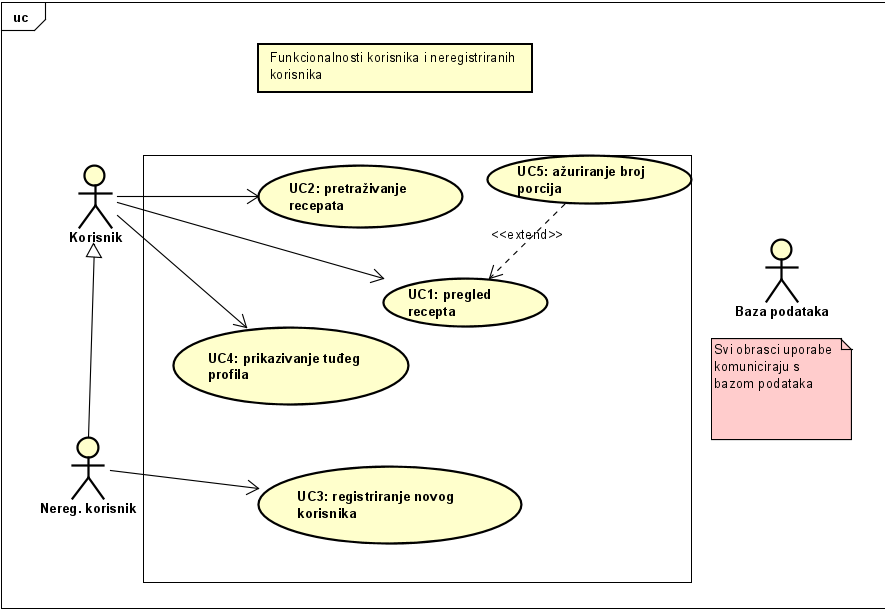
\includegraphics[scale=1.2]{slike/UC_nereg.png} %veličina slike u odnosu na originalnu datoteku i pozicija slike
						\centering
						\caption{Dijagram obrasca uporabe, funkcionalnost korisnika i neregistriranog korisnika}
						\label{fig:UC_diagram1}
					\end{figure}

					\begin{figure}[H]
						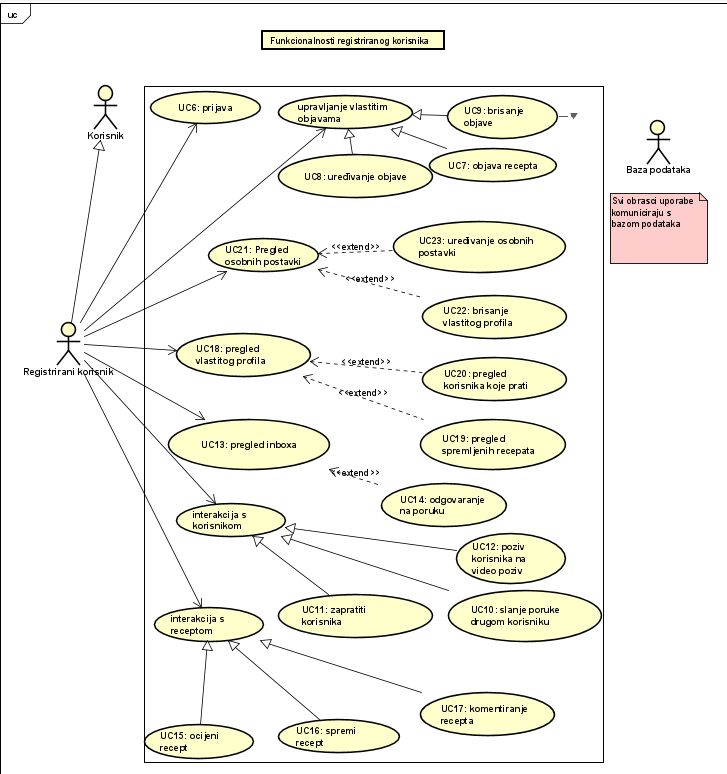
\includegraphics[scale=1.5]{slike/UC_reg.png} %veličina slike u odnosu na originalnu datoteku i pozicija slike
						\centering
						\caption{Dijagram obrasca uporabe, funkcionalnost registriranog korisnika}
						\label{fig:UC_diagram2}
					\end{figure}

					\begin{figure}[H]
						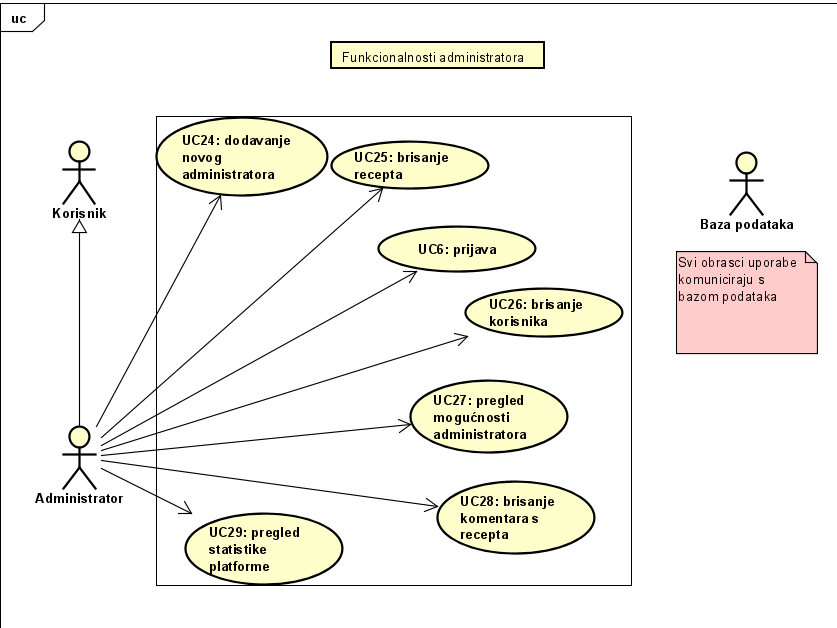
\includegraphics[scale=1.2]{slike/UC_admin.png} %veličina slike u odnosu na originalnu datoteku i pozicija slike
						\centering
						\caption{Dijagram obrasca uporabe, funkcionalnost administratora}
						\label{fig:UC_diagram3}
					\end{figure}
				\eject		
				
			\subsection{Sekvencijski dijagrami}
				
			\begin{figure}[H]
				\textbf{Obrazac uporabe UC3 - Registriranje novog korisnika}\\

				Neregistrirani korisnik šalje zahtjev za registraciju te mu web-aplikacija šalje odgovor formom za registraciju. Dokle god web-aplikacija u bazi podataka provjerom dobije odgovor da su email ili lozinka zauzeti korisnik dobiva poruku o zauzetosti emaila ili lozinke te ponovnu formu za upis podataka. Nakon unosa kod kojeg su email i username dostupni korisnikove informacije se zapisuju u bazu podataka. Korisnik dobiva poruku o uspješnoj registraciji.
				\begin{center}
					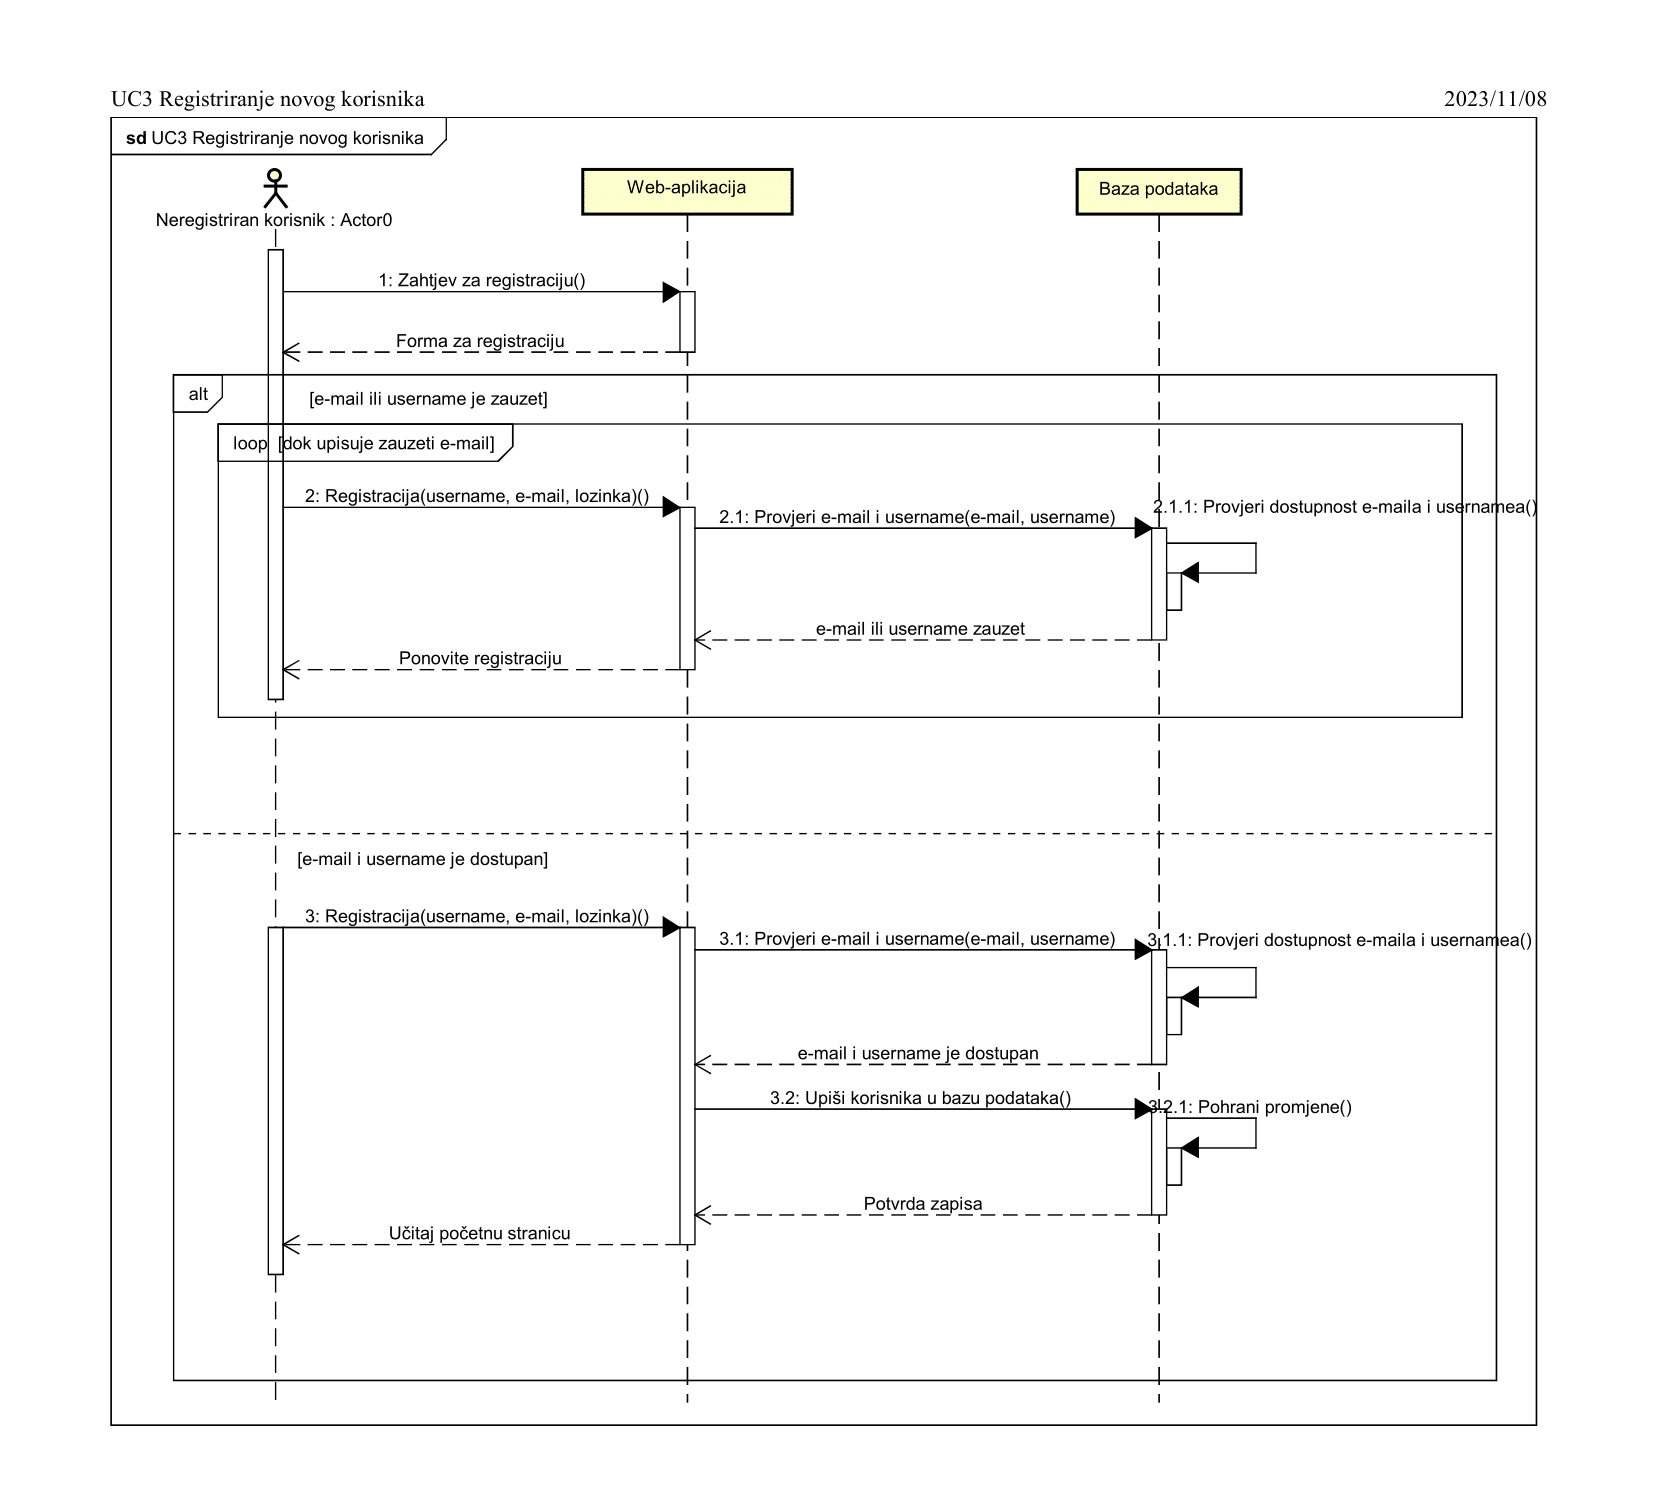
\includegraphics[scale = 0.8]{slike/SEK_UC3_Registriranje_novog_korisnika.png}
					\caption{Sekvencijski dijagram za UC3}
					\label{fig:Sek_UC3}
				\end{center}
			\end{figure}

			\begin{figure}[H]
				\textbf{Obrazac uporabe UC7 - Objava recepta}\\

				Registrirani korisnik šalje zahtjev za objavu recepte, a web-aplikacija mu odgovara formom za unos recepta. Registrirani korisnik unosi podatke o receptu: naslov, sastojci, priprema, vrijeme, kategorije, slike, video. Novonastali recept se zatim sprema u bazu podataka i web-aplikacija dobiva potvrdu o spremljenim podacima. Nakon potvrde web-aplikacija bazi podataka šalje zahtjev sa svim korisnicima koji su pratitelji autora objavljenog recepta te im svima šalje obavijest o novoj objavi.
				\begin{center}
					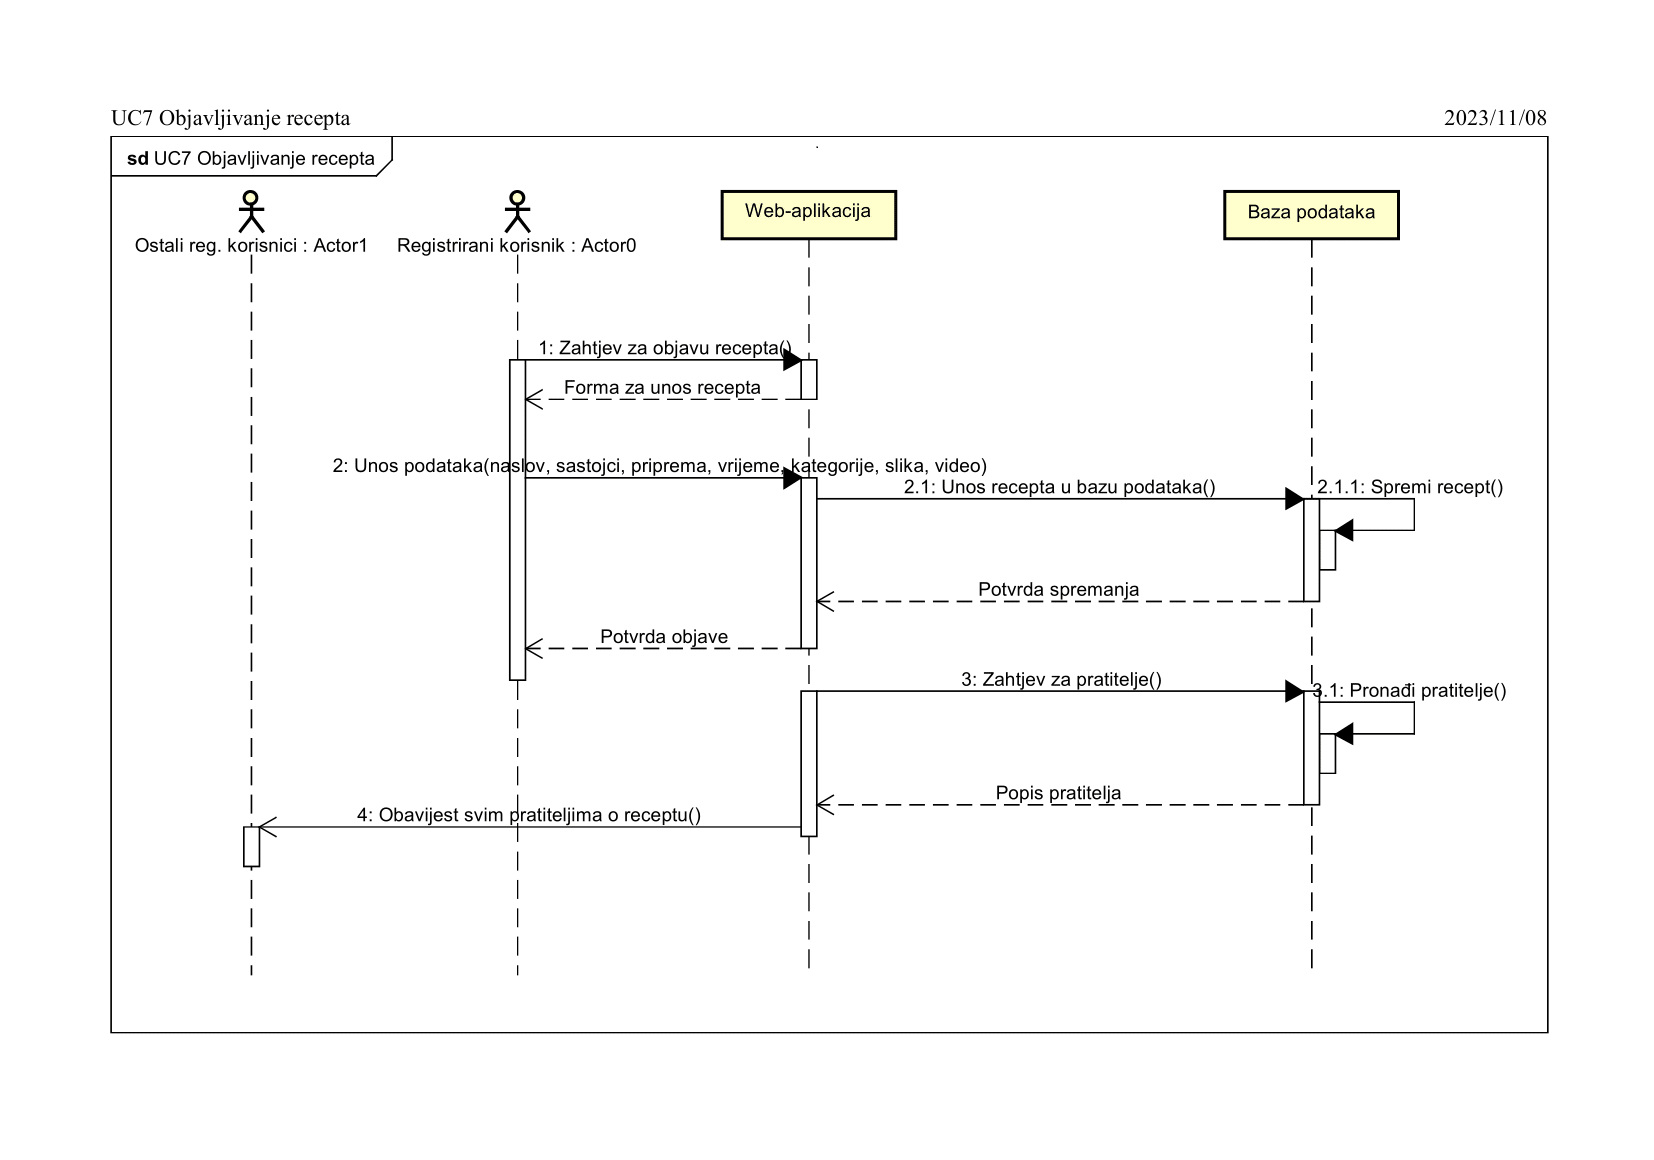
\includegraphics[scale = 0.8]{slike/SEK_UC7_Objavljivanje_recepta.png}
					\caption{Sekvencijski dijagram za UC7}
					\label{fig:Sek_UC7}							
				\end{center}
			\end{figure}

			\begin{figure}[H]
				\textbf{Obrazac uporabe UC18 - Pregled vlastitog profila}\\

				Registrirani korisnik šalje zahtjev za prikaz svog profila i web aplikaciju mu prikazuje sve informacije dobivene iz baze podataka. Nakon toga korisnik može zatražiti popis svih korisnika koji ga prate (UC20 Pregled profila koje korisnik prati), a web-aplikaciju bi mu odgovorila popisom korisnika koju bi dobila slanjem zahtjeva bazi podataka.
				Korisnik može odabrati i opciju pregledavanja spremljenih recepata (UC19 Pregledavanje spremljenih recepata) koji se prikazuju tako što web-aplikacija dobiva popis spremljenih recepata iz baze podataka.
				\begin{center}
					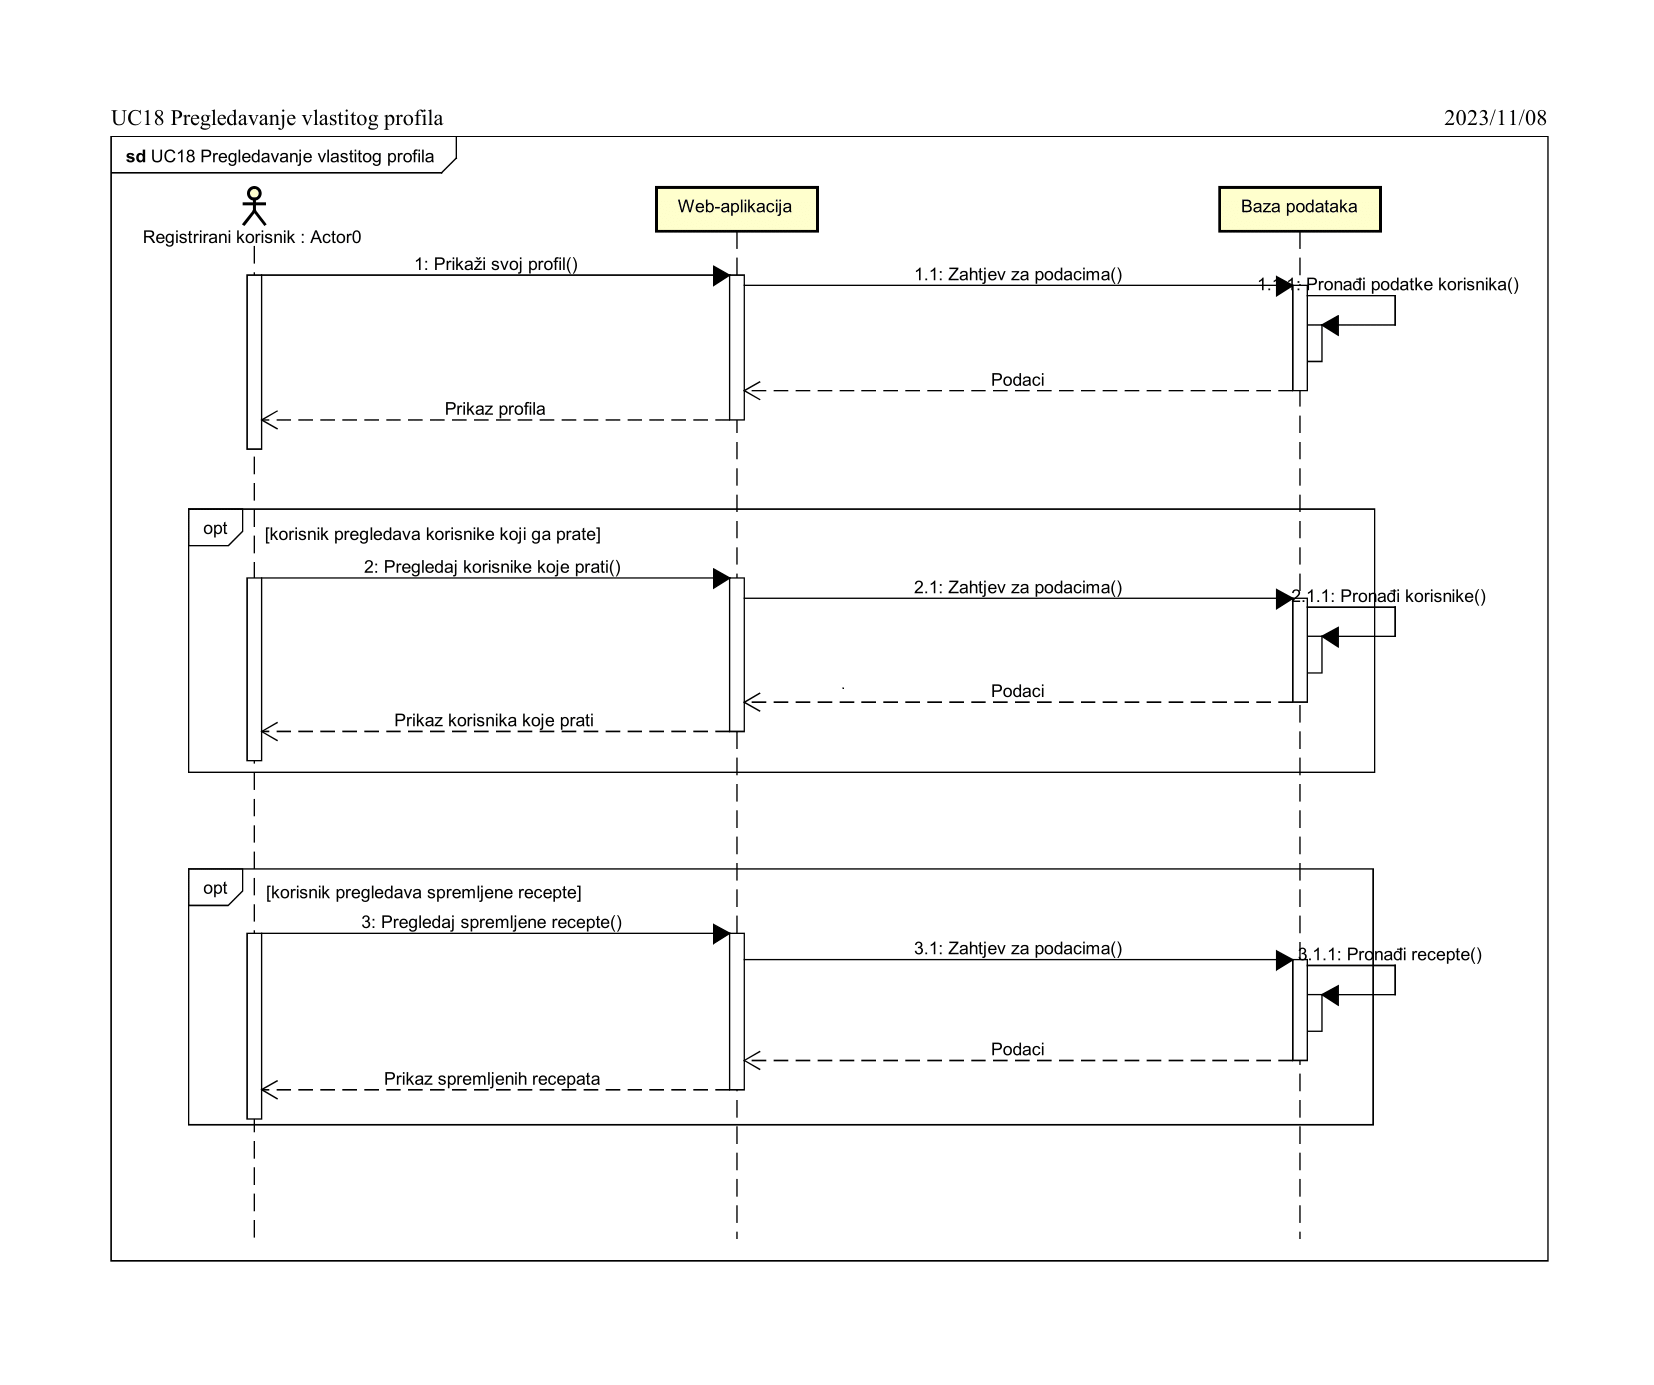
\includegraphics[scale = 0.8]{slike/SEK_UC18_Pregledavanje_vlastitog_profila.png}
					\caption{Sekvencijski dijagram za UC18}
					\label{fig:Sek_UC18}
				\end{center}
			\end{figure}

			\begin{figure}[H]
				\textbf{Obrazac uporabe UC21 - Pregled osobnih postavki}\\

				Registrirani korisnik šalje zahtjev za pregled osobnih postavki. Web-aplikacija prihvaća zahtjev i pošalje upit bazi podataka koja šalje sve podatke korisnika koje može ažurirati/brisati. Korisnik može odabrati opciju uređivanja profila (UC23 Uređivanje osobnih postavki), a web-aplikacija mu šalje formu za uređivanje postavki. Nakon što korisnik upiše promjene, potvrda promjena se šalje web-aplikaciji koja prosljeđuje podatke bazi podataka koja za tog korisnika ažurira promjene. Druga opcija koju korisnik može odabrati je brisanje profila (UC22 Brisanje vlastitog profila). Korisnik šalje zahtjev za brisanje profila web-aplikaciji koja prosljeđuje podatke korisnika bazi podataka koja ga na kraju briše.
				\begin{center}
					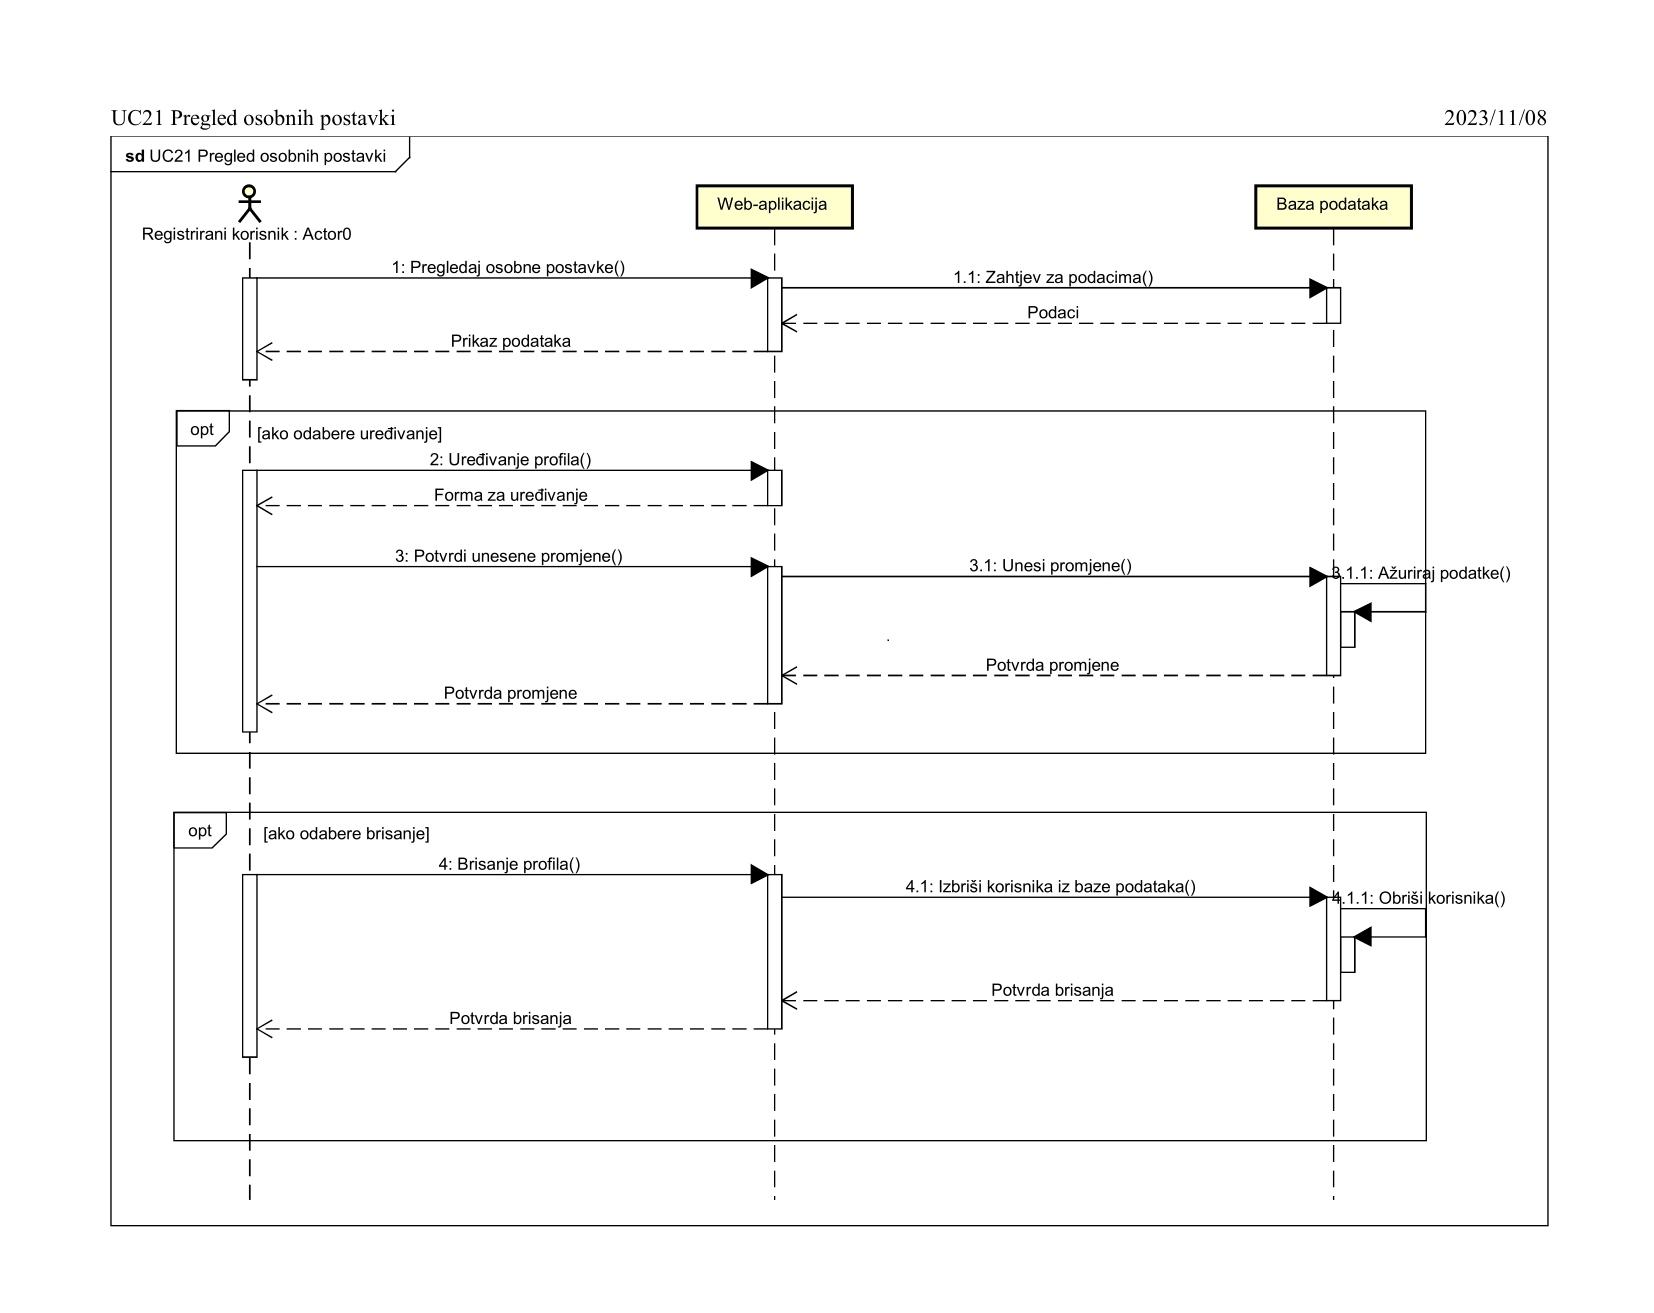
\includegraphics[scale = 0.8]{slike/SEK_UC21_Pregled_osobnih_postavki.png}
					\caption{Sekvencijski dijagram za UC21}
					\label{fig:Sek_UC21}
				\end{center}
			\end{figure}
				
			\eject
	
		\section{Ostali zahtjevi}
			 
			 \begin{packed_item}
			 	\item Aplikaciji se pristupa s pomoću internetskog preglednika korištenjem HTTPS protokola
			 	\item Aplikaciji treba moći pristupiti više korisnika istovremeno
			 	\item Korisničko sučelje mora biti intuitivno i jednostavno za korištenje
			 	\item Dizajn korisničkog sučelja mora biti responzivan kako bi se aplikaciji moglo pristupiti i s mobilnih uređaja
			 	\item Sustav mora biti otporan na greške uzrokovane neispravnim korištenjem korisničkog sučelja
			 	\item Postupak prijave korisnika mora biti siguran, a lozinke ne smiju biti pohranjene kao otvoreni tekst
			 	\item Baza podataka mora sadržavati odgovarajuće indekse kako bi pristup podatcima bio brz
			 	\item Baza podataka mora biti odvojena od ostatka sustava, ne smije joj se moći pristupiti izravno, već samo preko back-enda aplikacije
			 	\item Korisničko sučelje i baza podataka moraju podržavati dijakritičke znakove
			 	\item Pri implementaciji moraju biti korištena načela objektno-orijentiranog programiranja
			 	\item Razvojna verzija aplikacije mora biti u potpunosti odvojena od produkcijske kako rad na nadogradnjama ne bi utjecao na postojeće funkcionalnosti
			 	
			 \end{packed_item}
			 \eject
			 
			 
			 
	
	\chapter{Arhitektura i dizajn sustava}
		
	% 	\textbf{\textit{dio 1. revizije}}\\

	% 	\textit{ Potrebno je opisati stil arhitekture te identificirati: podsustave, preslikavanje na radnu platformu, spremišta podataka, mrežne protokole, globalni upravljački tok i sklopovsko-programske zahtjeve. Po točkama razraditi i popratiti odgovarajućim skicama:}
	% \begin{itemize}
	% 	\item 	\textit{izbor arhitekture temeljem principa oblikovanja pokazanih na predavanjima (objasniti zašto ste baš odabrali takvu arhitekturu)}
	% 	\item 	\textit{organizaciju sustava s najviše razine apstrakcije (npr. klijent-poslužitelj, baza podataka, datotečni sustav, grafičko sučelje)}
	% 	\item 	\textit{organizaciju aplikacije (npr. slojevi frontend i backend, MVC arhitektura) }		
	% \end{itemize}
		
		\section{Organizacija sustava}
			\subsection{Uvod}
				Arhitekturu sustava čine tri glavna dijela:
				\begin{packed_item}
					\item Baza podataka
					\item Aplikacijski front-end
					\item Aplikacijski back-end
				\end{packed_item}
			
				Front-end aplikacije ključan je dio u uspostavljanju komunikacije između korisnika i aplikacije. Korisnik aplikaciji pristupa uz pomoć internetskog preglednika na svom računalu, mobitelu ili nekom drugom uređaju. Preglednik komunicira s poslužiteljem preko HTTP protokola slanjem odgovarajućih zahtjeva. Front-end korisnikove zahtjeve zatim prosljeđuje back-endu koji predstavlja samu aplikaciju.
				\linebreak
				Aplikacija preuzima zahtjev te ga obrađuje sukladno njegovoj vrsti i parametrima. Obrada zahtjeva uključuje i pristupanje bazi podataka kako bi se dohvatili podatci potrebni za rad. Po završetku obrade zahtjeva, aplikacija front-endu vraća odgovor, a on ga dalje šalje korisniku.
				\linebreak
				Baza podataka može se nalaziti na istom računalu kao i ostali dijelovi sustava ili različitom, no komunikacija se uvijek odvija na isti način, preko dobro poznatih vrata na transportnom sloju i korištenjem odgovarajućeg protokola.
				\begin{figure}[H]
					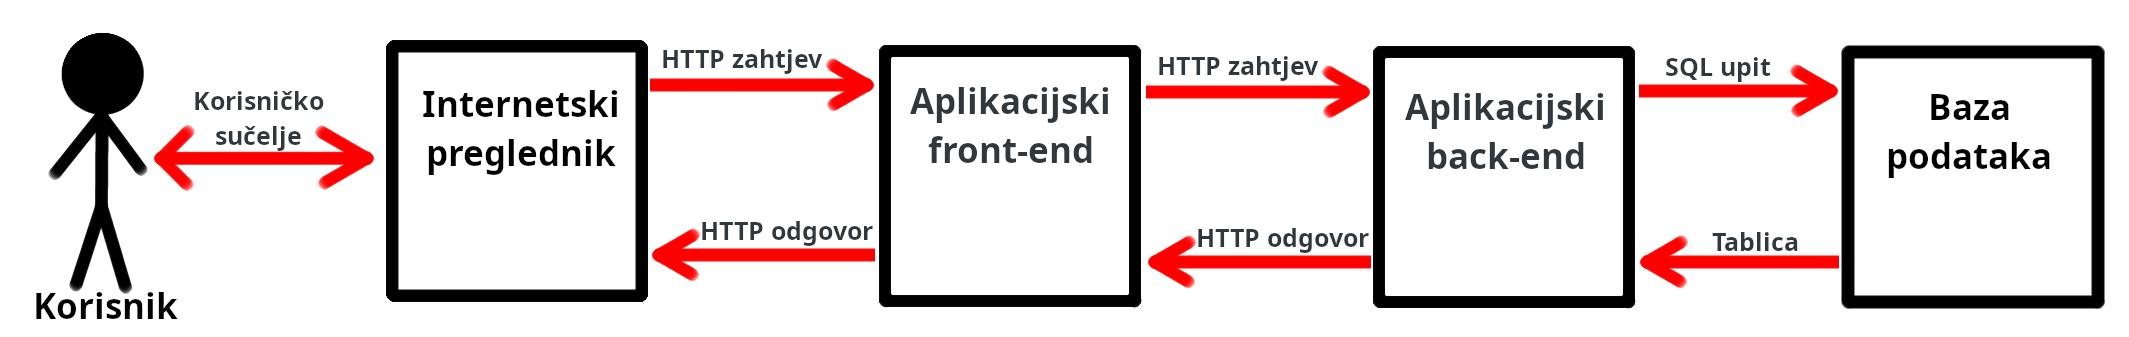
\includegraphics[scale=0.85]{slike/skica_arhitekture.png}
					\centering
					\caption{Arhitektura sustava}
					\label{fig:arhitektura_sustava}
				\end{figure}
			\subsection{Sklopovski zahtjevi}
				Ako se aplikacijski poslužitelj i baza podataka nalaze na različitim računalima, za optimalan rad ona bi trebala imati odgovarajuće karakteristike. Računalo na kojem će raditi poslužitelj treba imati dovoljnu veliku procesorsku moć kako bi moglo što brže odgovarati na zahtjeve i kako bi više korisnika moglo koristiti aplikaciju bez značajnog usporavanja sustava. Računalo na kojem će se nalaziti baza podataka treba imati dovoljno velike i brze diskove za pohranu podataka, idealno uz neku vrstu zaštite od gubitka podataka u slučaju kvara (na primjer, korištenje RAID sustava ili automatskog redovitog stvaranja sigurnosne kopije). Ako se pak poslužitelj i baza podataka pokreću na istom računalu, ono treba kombinirati maloprije navedene karakteristike.
			\subsection{Organizacija aplikacije}
				Za izradu aplikacije odabrani su programski jezik Java uz razvojni okvir Spring te Javascript i razvojni okvir React. Dva glavna sloja aplikacije su frontend, koji komunicira s korisnikom (Javascript + React) i backend, koji obrađuje HTTP zahtjeve i komunicira s bazom podataka (Java + Spring).
				%U primjeru dokumentacije oni ovdje jos pisu da se arhitektura temelji na MVCu i to dodatno opisuju
				%Ovaj dio bi onda trebali dovrsit kada vidimo sto cemo s time
				
				
		

				\section{Baza podataka}
			
				Naš će sustav koristiti relacijsku bazu podataka čija je osnovna jedinica baze relacija, odnosno tablica, koja je definirana svojim imenom i skupom atributa. Baza podataka ima zadatak brzo i jednostavno pohranjivati, mijenjati i dohvaćati podatke za daljnju obradu. Baza podataka stranice sastoji se od sljedećih entiteta:
				 \begin{packed_item}
					 \item Korisnik
					 \item Recept
					 \item Oznaka
						 \item Komentar
					 \item Ocjena
					 \item Poruka
						 \item Sastojak
				 \end{packed_item}
		 
			 \subsection{Opis tablica}
			 
 
				 \textbf{Korisnik} Ovaj entitet sadržava sve važne informacije o korisniku aplikacije. Sadrži atribute: Korisničko ime, lozinku, ime, prezime, razinu ovlasti korisnika i e-mail korisnika. Ovaj entitet u vezi je \textit{One-to-Many} s entitetima Recept, Komentar i Ocjena te je s entitetom poruka u ulozi primatelj i pošiljatelj isto u \textit{One-to-Many} vezi, sve preko ID-a korisnika.
				 
				 
				 \begin{longtblr}[
					 label=none,
					 entry=none
					 ]{
						 width = \textwidth,
						 colspec={|X[8,l]|X[8, l]|X[18, l]|}, 
						 rowhead = 1,
					 } %definicija širine tablice, širine stupaca, poravnanje i broja redaka naslova tablice
					 \hline \SetCell[c=3]{c}{\textbf{Korisnik}}	 \\ \hline[3pt]
					 \SetCell{LightGreen} ID Korisnika	& INT &  jedinstveni identifikator korisnika\\ \hline 
					 Lozinka & VARCHAR	&  lozinka korisnika	\\ \hline 
						 Korisničko ime & VARCHAR	&  korisničko ime	\\ \hline 
						 Ime & VARCHAR	& ime korisnika\\ \hline 
					 Prezime & VARCHAR &  prezime korisnika \\ \hline 
						 Razina Ovlasti & VARCHAR &  razina ovlasti korisnika \\ \hline 
					 Email & VARCHAR & e-mail adresa korisnika 	\\ \hline 
				 \end{longtblr}
				 
				 \textbf{Pretplata} Ovaj entitet sadrži informacije vezane za praćenje korisnika. Njegovi atributi su: ID korisnika kojeg se prati (praćenik), ID pratitelja i ID pretplate. Entitet je u \textit{Many-to-Many} vezi s korisnikom preko ID-a pratitelja i praćenika.
				 
				 \begin{longtblr}[
				 	label=none,
				 	entry=none
				 	]{
				 		width = \textwidth,
				 		colspec={|X[8,l]|X[8, l]|X[18, l]|},
				 		rowhead=1
				 	}
				 		\hline \SetCell[c=3]{c}{\textbf{Pretplata}}	 \\ \hline[3pt]
				 		\SetCell{LightGreen} IDpretplata	& INT &  jedinstveni identifikator pretplate \\ \hline 
				 		ID pratitelj & INT	&  ID korisnika koji prati	\\ \hline 
				 		ID praćenik & INT	&  ID korisnika kojeg se prati	\\ \hline 
				 \end{longtblr}
				 
				 \textbf{Recept} Ovaj entitet sadržava sve važne informacije o receptu. Sadrži atribute: ID recepta, naziv recepta, vrijeme pripreme, postupak pripreme, opis recepta, sliku recepta, datum recepta  i vrijeme objave recepta i prosječnu ocjenu recepta. Recept je u vezi \textit{Many-to-One} s korisnikom koji ga je objavio, u vezi \textit{One-to-Many} s ocjenom, sastojkom u receptu i komentarom preko ID-a recepta te u \textit{Many-to-Many} s oznakom recepta preko ID-a oznake.
				 
				 \begin{longtblr}[
					 label=none,
					 entry=none
					 ]{
						 width = \textwidth,
						 colspec={|X[8,l]|X[8, l]|X[18, l]|}, 
						 rowhead = 1,
					 } %definicija širine tablice, širine stupaca, poravnanje i broja redaka naslova tablice
					 \hline \SetCell[c=3]{c}{\textbf{Recept}}	 \\ \hline[3pt]
					 \SetCell{LightGreen}ID Recepta & INT	&  	jedinstveni identifikator recepta  	\\ \hline
					 Naziv recepta	& VARCHAR &   naziv recepta	\\ \hline 
					 Vrijeme pripreme & INTERVAL & vrijeme pripreme  \\ \hline 
					 Postupak pripreme & VARCHAR	& postupak pripreme\\ \hline 
					 Opis recepta & VARCHAR & opis recepta \\ \hline 
					 Slika recepta & LONGBOB	&  slika recepta	\\ \hline 
						 Datum i vrijeme recepta	& DATETIME & datum recepta  i vrijeme objave recepta 	\\ \hline 
						 Prosječna ocjena recepta	& INT &   prosječna ocjena recepta	\\ 
						 \hline
						 \SetCell{LightBlue} ID Korisnika	& INT &  ID korisnika koji je objavio recept\\ \hline 
						 \SetCell{LightBlue} ID oznake	& INT &  ID oznake recepta\\ \hline 
				 \end{longtblr}
 
				 \textbf{Oznaka} Ovaj entitet sadržava sve važne informacije o oznaci recepta. Sadrži atribute: ID oznake i naziv oznake. Oznaka je u \textit{Many-to-Many} vezi s receptom preko ID-a oznake.
	 
				 \begin{longtblr}[
					 label=none,
					 entry=none
					 ]{
						 width = \textwidth,
						 colspec={|X[8,l]|X[8, l]|X[18, l]|}, 
						 rowhead = 1,
					 } %definicija širine tablice, širine stupaca, poravnanje i broja redaka naslova tablice
					 \hline \SetCell[c=3]{c}{\textbf{Oznaka}}	 \\ \hline[3pt]
					 \SetCell{LightGreen}ID oznake & INT	&  	jedinstveni identifikator oznake  	\\ \hline
					 Naziv oznake & VARCHAR & naziv oznake  	\\ \hline 
				 \end{longtblr}
 
				 \textbf{Komentar} Ovaj entitet sadržava sve važne informacije o komentaru recepta. Sadrži atribute: ID komentara, ID komentatora, ID recepta, tekst komentara i datum i vrijeme komentara. Komentar je u \textit{Many-to-One} vezi s korisnikom preko ID-a korisnika koji ga objavi i receptom preko ID-a recepta. 
 
				 \begin{longtblr}[
					 label=none,
					 entry=none
					 ]{
						 width = \textwidth,
						 colspec={|X[8,l]|X[8, l]|X[18, l]|}, 
						 rowhead = 1,
					 } %definicija širine tablice, širine stupaca, poravnanje i broja redaka naslova tablice
					 \hline \SetCell[c=3]{c}{\textbf{Komentar}}	 \\ \hline[3pt]
						 \SetCell{LightGreen}ID komentar & INT &  ID komentara	\\ \hline
					 Tekst komentara	& VARCHAR &  tekst komentara 	\\ \hline 
						 ID komentatora	& INT &  ID korisnika komentatora	\\ \hline
						 ID recepta	& INT &  ID recepta na kojem je komentar postavljen	\\ \hline
						 Datum i vrijeme komentara	& DATETIME &  datum i vrijeme komentara	\\ \hline 
				 \end{longtblr}
 
				 \textbf{Ocjena} Ovaj entitet sadržava sve važne informacije o pojedinoj ocjeni recepta. Sadrži atribute: ID ocjenitelja, ID recepta i datum i vrijeme ocjene. Entitet je u vezi \textit{Many-to-One} s ocjeniteljem preko ID-a korisnika koji je ocijenio recept i \textit{Many-to-One} s receptom preko ID-a recepta.
 
				 \begin{longtblr}[
					 label=none,
					 entry=none
					 ]{
						 width = \textwidth,
						 colspec={|X[8,l]|X[8, l]|X[18, l]|}, 
						 rowhead = 1,
					 } %definicija širine tablice, širine stupaca, poravnanje i broja redaka naslova tablice
					 \hline \SetCell[c=3]{c}{\textbf{Ocjena}}	 \\ \hline[3pt]
					 Ocjena	& VARCHAR & ocjena	\\ \hline
						 \SetCell{LightBlue}ID ocjenitelja	& INT &  ID korisnika koji je ostavio poruku	\\ \hline
						 \SetCell{LightBlue}ID recepta	& INT &  ID recepta koji je ocjenjen	\\ \hline
						 Datum i vrijeme ocjene	& DATETIME &  datum i vrijeme ocjene	\\ \hline 
				 \end{longtblr}
 
				 \textbf{Poruka} Ovaj entitet sadržava sve važne informacije o poruci između dva korisnika. Sadrži atribute: ID poruke, ID pošiljatelja, ID primatelja, tekst poruke i datum i vrijeme poruke. Poruka je u vezi \textit{Many-to-One} s primateljem i pošiljateljem preko ID-a korisnika koji palje i prima poruku.
 
				 \begin{longtblr}[
					 label=none,
					 entry=none
					 ]{
						 width = \textwidth,
						 colspec={|X[8,l]|X[8, l]|X[18, l]|}, 
						 rowhead = 1,
					 } %definicija širine tablice, širine stupaca, poravnanje i broja redaka naslova tablice
					 \hline \SetCell[c=3]{c}{\textbf{Poruka}}	 \\ \hline[3pt]
						 \SetCell{LightGreen}ID Poruka	& INT &  ID poruka \\ \hline
					 Tekst poruka & VARCHAR & tekst poruka  	\\ \hline 
						 ID pošiljatelja	& INT &  ID korisnika koji šalje poruku	\\ \hline 
						 ID primatelja	& INT & ID korisnika koji prima poruku	\\ \hline 
						 Datum i vrijeme poruke & TIMESTAMP &  datum i vrijeme poruke	\\ \hline 
				 \end{longtblr}
 
				 \textbf{Sastojak} Ovaj entitet sadržava sve važne informacije o sastojku navedenom u nekom receptu. Sadrži atribute: ID sastojka, naziv sastojka. Entitet je u vezi \textit{Many-to-Many} sa sastojkom u receptu preko ID-a recepta.
 
				 \begin{longtblr}[
					 label=none,
					 entry=none
					 ]{
						 width = \textwidth,
						 colspec={|X[8,l]|X[8, l]|X[18, l]|}, 
						 rowhead = 1,
					 } %definicija širine tablice, širine stupaca, poravnanje i broja redaka naslova tablice
					 %Zašto imamo IDSastojak? Jer može biti više sastojaka s istim imenom, istom količinom u istom receptu (npr 100 ml mlijeka u kremi i 100 ml mlijeka u tjestu)
					 \hline \SetCell[c=3]{c}{\textbf{Sastojak}}	 \\ \hline[3pt]
						 \SetCell{LightGreen}ID Sastojka	& INT &  ID sastojka \\ \hline
						 Naziv sastojka	& VARCHAR &  naziv sastojka	\\ \hline
					 
				 \end{longtblr}
 
				 \textbf{Sastojak u receptu} Ovaj entitet sadržava sve važne informacije o sastojku navedenom u nekom receptu. Sadrži atribute: ID sastojka, ID recepta, količinu. Entitet je u vezi \textit{Many-to-One} s receptom preko ID-a recepta i u vezi \textit{Many-to-Many} sa sastojkom preko ID sastojak.
				 
				 \begin{longtblr}[
					 label=none,
					 entry=none
					 ]{
						 width = \textwidth,
						 colspec={|X[8,l]|X[8, l]|X[18, l]|}, 
						 rowhead = 1,
					 } %definicija širine tablice, širine stupaca, poravnanje i broja redaka naslova tablice
					 %Zašto imamo IDSastojak? Jer može biti više sastojaka s istim imenom, istom količinom u istom receptu (npr 100 ml mlijeka u kremi i 100 ml mlijeka u tjestu)
					 \hline \SetCell[c=3]{c}{\textbf{Sastojak u receptu}}	 \\ \hline[3pt]
						 \SetCell{LightBlue}ID Sastojka	& INT &  ID sastojka \\ \hline
						 \SetCell{LightBlue}ID recepta	& INT &   ID recepta u kojem je sastojak	\\ \hline
						 Količina	& VARCHAR &   količina	\\ \hline
					 
				 \end{longtblr}
				 
			 
			 \subsection{Dijagram baze podataka}
			 \begin{figure}[H]
				 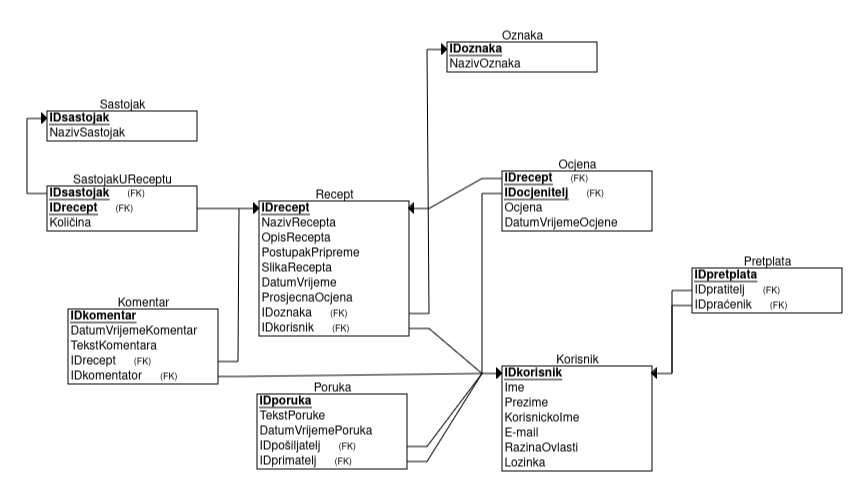
\includegraphics[scale=0.50]{slike/dijagram_baze_v2.png} %veličina slike u odnosu na originalnu datoteku i pozicija slike
				 \centering
				 \caption{Relacijski dijagram baze podataka}
				 \label{fig:Relacijski dijagram baze podataka}
			 \end{figure}
		 
			 \eject
			
			
		\section{Dijagram razreda}

		Prvi dijagram prikazuje trenutno stanje stranice. Dijagram ima jedan repozitorij, entitet i servis te 5 kontrolera.
		\begin{figure}[H]
			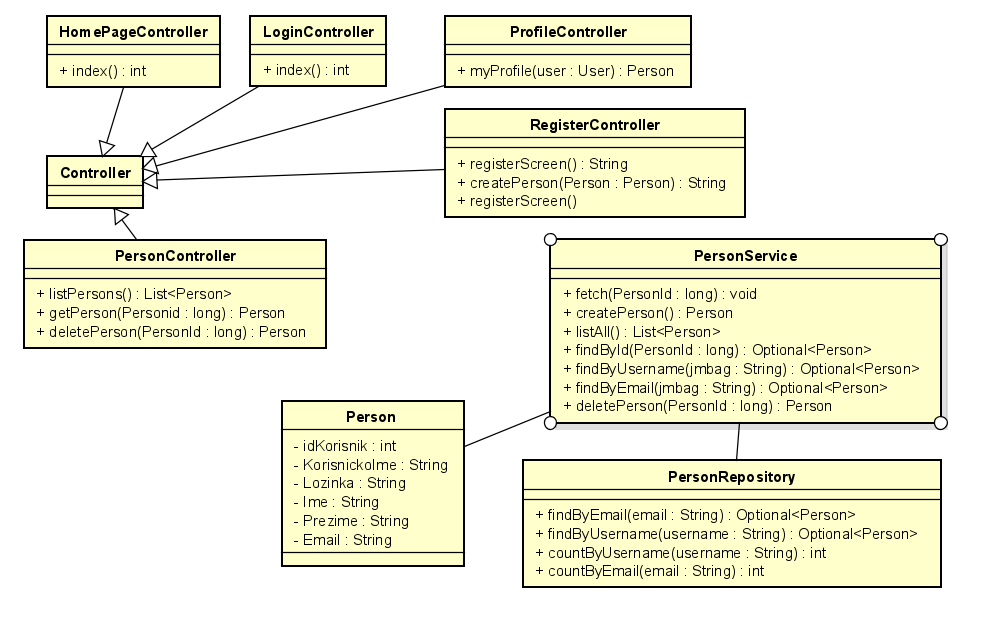
\includegraphics[scale=0.75]{slike/dijagram_razreda2.png} %veličina slike u odnosu na originalnu datoteku i pozicija slike
			\centering
			\caption{Dijagram razreda - dio Controllers}
			\label{fig:Dijagram_razreda2}
		\end{figure}


		Drugi dijagram prikazuje glavne entitete i veze između njih, 
		tj. preslikava strukturu baze podataka. Razred Korisnik 
		predstavlja neregistriranog korisnika koji se može registrirati 
		u Razred RegistriraniKorisnik predstavlja korisnika koji je registriran u sustav 
		i koji može koristiti više od osnovnih funkcija korisnika. NeRegistriraniKorisnik predstavlja vrstu korisnika i može se registrirati.
		Razred Administrator predstavlja administratora sustava koji ima najveće ovlasti. 



		\begin{figure}[H]
			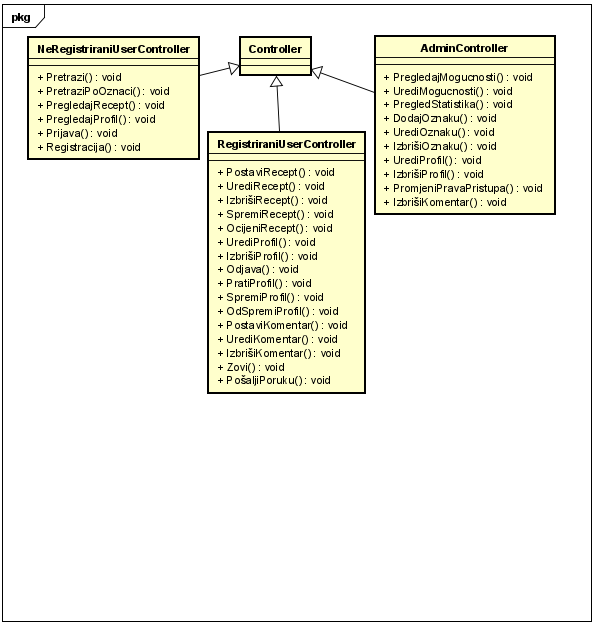
\includegraphics[scale=1.3]{slike/dijagram_razreda1.png} %veličina slike u odnosu na originalnu datoteku i pozicija slike
			\centering
			\caption{Dijagram razreda - dio Data transfer objects}
			\label{fig:Dijagram_razreda1}
		\end{figure}
			
			
			\eject
		
		\section{Dijagram stanja}
			
			
			% \textbf{\textit{dio 2. revizije}}\\
			
			% \textit{Potrebno je priložiti dijagram stanja i opisati ga. Dovoljan je jedan dijagram stanja koji prikazuje \textbf{značajan dio funkcionalnosti} sustava. Na primjer, stanja korisničkog sučelja i tijek korištenja neke ključne funkcionalnosti jesu značajan dio sustava, a registracija i prijava nisu. }
			Dijagram stanja na slici \ref{fig:Dijagram_stanja} opisuje stanja u kojima se registrirani korisnik može naći i njihove okidače te prijelaze. Nakon uspješne prijave, korisniku se prikazuje početna stranica na kojoj može pretražiti recept pomoću tražilice, pregledati svoj pretinac poruka, pregledati svoj profil, objaviti recept ili pogledati nove recepte koje su objavili korisnici koje prati. Na vlastitom profilu se prikazuju osobni podaci, objavljeni recepti i gumbovi za dodatne mogućnosti. Dodatne funkcionalnosti na stranici profila su opcije za daljnji pregled osobnih postavki, prikaz spremljenih recepata i prikaz korisnika koje prati. Klikom na "Postavke" korisnik može ažurirati svoje podatke ili obrisati svoj račun. Klikom na "Pretinac poruka" prikazuju se izmijenjene poruke. U pretincu se može otvoriti poruka njezinim odabirom te poslati nova poruka, čime se pritiskom gumba otvara šablona za poruku. Odabirom opcije "Objavi recept" otvara se nova stranica na kojoj se nalazi šablona za stvaranje recepta. Upisivanjem ključnih riječi u tražilicu prikaže se stranica s receptima koji se poklapaju s danim opisom. Odabirom recepta otvara se pojedinačna stranica sa samo odabranim receptom. Na stranici pregleda recepta korisnik može ocijeniti, spremiti ili komentirati recept, u slučaju da je korisnik autor prikazanog recepta pojavljuje se opcija uređivanja ili brisanja recepta. Korisnik također može pritisnuti na korisničko ime korisnika koji je objavio recept, time se otvara stranica tuđeg profila. Prikazivanjem tuđeg profila moguće je zapratiti korisnika ili poslati privatnu poruku korisniku, čime se ponovno otvara šablona za poruku. Korisnik uvijek ima mogućnost povratka na početnu stranicu, otvaranja pretinca poruka, pregleda korisničkog profila, pregleda novosti i objavljivanja recepta.
			\begin{figure}[H]
				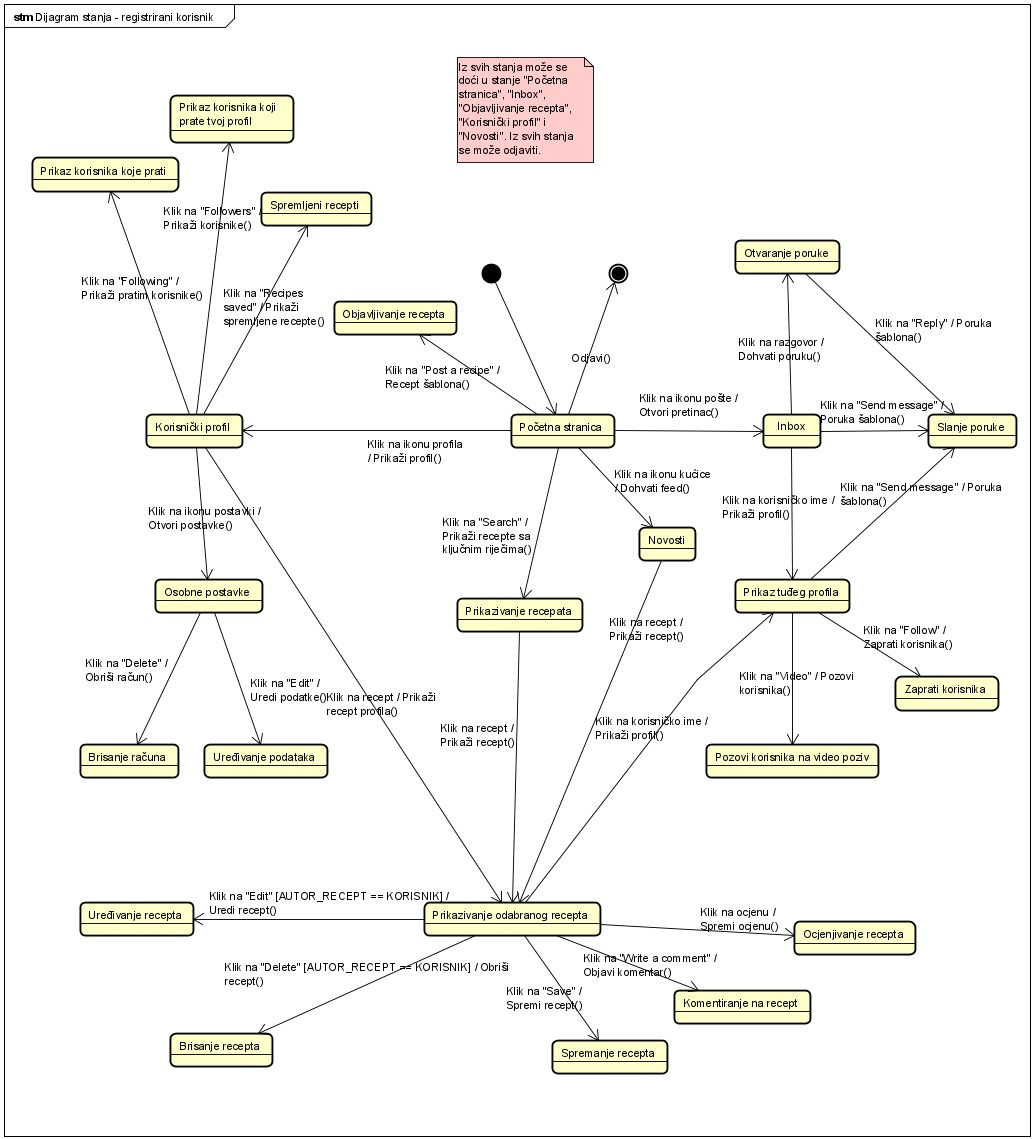
\includegraphics[scale=0.5]{slike/dijagram_stanja.jpeg} %veličina slike u odnosu na originalnu datoteku i pozicija slike
				\centering
				\caption{Dijagram stanja - registrirani korisnik}
				\label{fig:Dijagram_stanja}
			\end{figure}
			
			\eject 
		
		\section{Dijagram aktivnosti}
			
			%\textbf{\textit{dio 2. revizije}}\\
			
			 %\textit{Potrebno je priložiti dijagram aktivnosti s pripadajućim opisom. Dijagram aktivnosti treba prikazivati značajan dio sustava.}
			 Dijagram aktivnosti u nastavku prikazuje tok upravljanja jedne od najvažnijih funkcionalnosti stranice, a to je objava novog recepta. Dva glavna sudionika su korisnik koji objavljuje recept te baza podataka u koju se zapisuje, a cijelim postupkom upravlja sama aplikacija, odnosno back-end. Dijagram je sukladno tome podijeljen na tri particije.
			 
			 Korisnik se najprije mora prijaviti u aplikaciju. Nakon uspješne prijave prikazuje mu se početna stranica s koje korisnik može odabrati opciju za objavu novog recepta. Odabirom te opcije otvara se novi prozor te korisnik može započeti s pisanjem recepta. Nakon što je korisnik gotov s pisanjem, back-end provjerava sadrži li recept sve potrebne podatke. Ako je recept valjan, upisuje ga se u bazu podataka te se na kraju korisnicima koji prate autora u obliku poruke šalje obavijest o novoj objavi.
			 \begin{figure}
			 	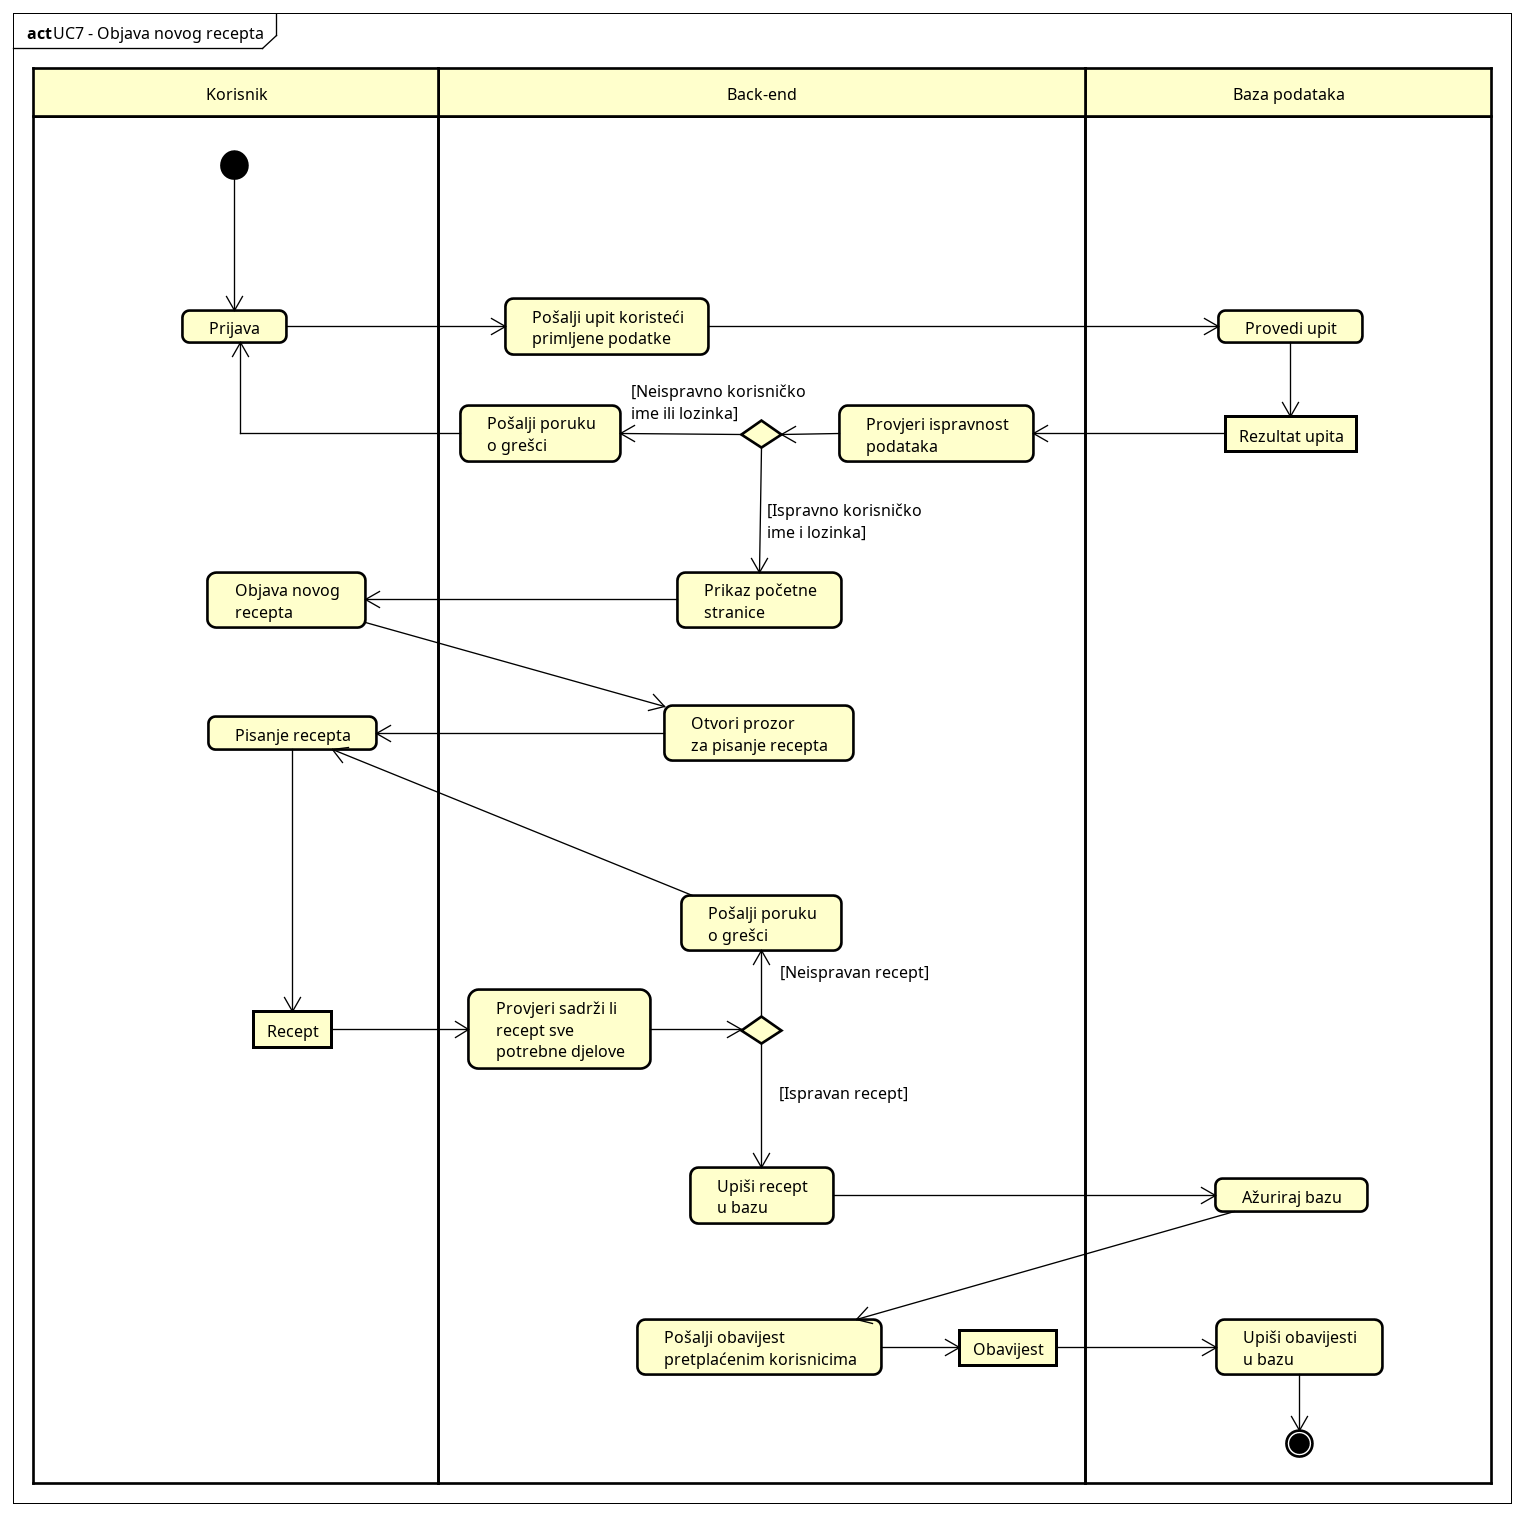
\includegraphics[scale=0.41]{slike/dijagram_aktivnosti.png}
			 	\centering
			 	\caption{Dijagram aktivnosti objave novog recepta}
			 	\label{fig:Dijagram_aktivnosti objave novog recepta}
			 \end{figure}
			 
			\eject
		\section{Dijagram komponenti}
		
			Slika \ref{fig:dijagram_komponenti} pruža prikaz organizacije komponenata, internih struktura, njihovih međusobnih odnosa te njihovih veza s okolinom.
			Spring Boot korišten pri izradi aplikacije, koristi se za brzu i lagano pokretljivu izgradnju servera koji obrađuje HTTP zahtjeve putem definiranih REST API endpointa.
			Preko sučelja za dohvat HTML, CSS i JS datoteka poslužuju se datoteke koje pripadaju frontend dijelu aplikacije. App.js, tj. Router omogućava navigaciju između različitih stranica, Home, Login, Register, Profile i AdminPage. To je komponenta koja na upit s url određuje koja datoteka će se poslužiti na sučelje.
			Na korisnički zahtjev Korisnik interaktira s frontend-om, pokrećući HTTP zahtjeve prema backend API-ju. API endpointi u kontrolerima backend-a prihvaćaju i vraćaju DTO-ove. DTO-ovi se koriste kako bi podatke omotali na način koji ima smisla za frontend, ne izlažući pritom unutarnji podatkovni model backend-a. Repozitoriji omogućavaju interakciju s H2 in-memory bazom podataka. Ona se koristi za pohranu podataka tijekom trajanja aplikacije. Automatski se stvara prilikom pokretanja backend-a i nestaje nakon gašenja. Dakle, backend prima zahtjev, obrađuje ga putem odgovarajućih kontrolera i servisa i ako je potrebno komunicira s H2 bazom podataka putem Repozitoriija. Backend onda generira odgovor u JSON formatu i šalje ga frontend-u koji ažurira svoje stanje i reagira na promjene korisničkog sučelja.
			\begin{figure}
				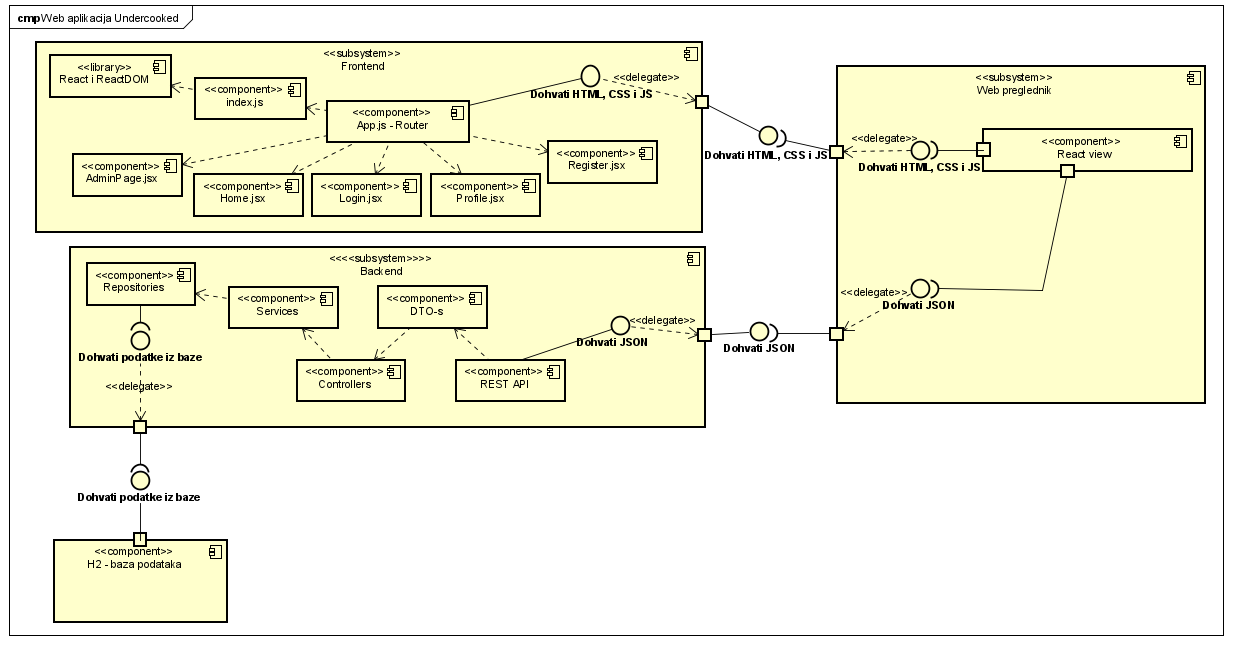
\includegraphics[scale=0.57]{slike/dijagram_komponenti.png}
				\centering
				\caption{Dijagram komponenti}
				\label{fig:dijagram_komponenti}
			\end{figure}
	\chapter{Implementacija i korisničko sučelje}
		
		
		\section{Korištene tehnologije i alati}
		
			\indent \indent Komunikacija grupe se odvijala putem aplikacije \href{https://www.whatsapp.com/}{WhatsApp\footnote{https://www.whatsapp.com/}}, dok je za održavanje sastanaka na daljinu korištena aplikacija \href{https://www.microsoft.com/en-us/microsoft-teams/group-chat-software/}{MicrosoftTeams\footnote{https://www.microsoft.com/en-us/microsoft-teams/group-chat-software/}}, koja pruža opciju video poziva. Sustav \href{https://git-scm.com/}{Git\footnote{https://git-scm.com/}} je omogućio upravljanje različitim verzijama programskog koda i dokumentacije uz udaljeni repozitorij na web platformi \href{https://github.com/}{GitHub\footnote{https://github.com/}}. Dokumentacija je pisana u programskom jeziku \href{https://www.latex-project.org/}{LaTeX\footnote{https://www.latex-project.org/}}, a za izradu UML dijagrama korišteni su alati \href{https://erdplus.com/}{ERDPlus\footnote{https://erdplus.com/}} i \href{https://astah.net/products/astah-uml/}{Astah UML\footnote{https://astah.net/products/astah-uml/}} sa studentskom licencom.
				
			\indent Korištena je kombinacija razvojnih okruženja ovisno o developeru. Aplikacija je napisana koristeći \href{https://eclipseide.org/}{Eclipse IDE\footnote{https://eclipseide.org/}} i \href{https://www.jetbrains.com/idea/}{IntelliJ IDEA\footnote{https://www.jetbrains.com/idea/}}, dok je za pisanje dokumentacije korišteno razvojno okruženje \href{https://code.visualstudio.com/}{Visual Studio Code\footnote{https://code.visualstudio.com/}}. Eclipse je \textit{open-source} integrirano razvojno okruženje koje se dominantno koristi za razvoj Java aplikacija uz Java razvojne alate. Moguće je prilagoditi okruženje za razvoj web-stranica, web-aplikacija i mobilnih aplikacija uz alate za razvoj programskih aplikacija. Intellij IDEA je integrirano razvojno okruženje tvrtke JetBrains za razvoj računalnih programa u Javi, Kotlinu te drugim programskim jezicima koji se oslanjaju na Java virtualni stroj. Sadrži brojne značajke koje znatno olakšavaju pisanje aplikacija kao što su posebni alati za radne okvire Spring i Spring Boot, pametno popunjavanje koda i podrška pri radu s HTTP porukama. Visual Studio Code je integrirano razvojno okruženje tvrtke Microsoft koje se koristi za razvoj računalnih programa u brojnim računalnim jezicima poput Python, C/C++ i Java. Sva korištena razvojna okruženja su podržana na operacijskim sustavima Microsoft, Linux i macOS. \\
				
			\indent Aplikacija je napravljena u radnom okviru \href{https://spring.io/projects/spring-boot/}{Spring Boot\footnote{https://spring.io/projects/spring-boot/}} kao \href{https://maven.apache.org/}{Maven\footnote{https://maven.apache.org/}} projekt. Za izradu \textit{backenda} aplikacije korišten je programski jezik \href{https://www.java.com/en/}{Java\footnote{https://www.java.com/en/}}, a za izradu \textit{frontenda} je korišten \href{https://react.dev/}{React\footnote{https://react.dev/}} i programski jezik \href{https://www.javascript.com/}{JavaScript\footnote{https://www.javascript.com/}}. Spring Boot je specijalizacija radnog okvira Spring koji se temelji na višeslojnoj arhitekturi čiji je cilj ubrzati i pojednostaviti razvoj web-aplikacija. Spring boot pruža podršku za automatsko definiranje programskih zahtjeva prilikom stvaranja projekata, za ugrađeni server Tomcat i za bazu podataka. Maven je programska podrška za organizaciju projekata i automatizaciju pokretanja aplikacija. Koristimo \textit{in-memory} \href{https://www.h2database.com/html/main.html}{H2\footnote{https://www.h2database.com/html/main.html}} bazu podataka koju pruža Spring Boot. React je biblioteka u JavaScriptu za izgradnju korisničkih sučelja temeljenih na komponentama koju održava Facebook. Glavne značajke React-a su ponovno korištenje web komponenti i ponovno prikazivanje samo komponente koje su promijenjene, a ne cijelu stranicu. Uspostava sobe za video poziv je omogućena preko \href{https://www.daily.co/}{Daily\footnote{https://www.daily.co/}} WebRTC usluga. Ispitivanje projekta je provedeno pomoću \href{https://www.selenium.dev/documentation/webdriver/}{Selenium WebDriver\footnote{https://www.selenium.dev/documentation/webdriver/}}.

		\eject 
		
	
		\section{Ispitivanje programskog rješenja}
			
			\textbf{\textit{dio 2. revizije}}\\
			
			 \textit{U ovom poglavlju je potrebno opisati provedbu ispitivanja implementiranih funkcionalnosti na razini komponenti i na razini cijelog sustava s prikazom odabranih ispitnih slučajeva. Studenti trebaju ispitati temeljnu funkcionalnost i rubne uvjete.}
	
			
			\subsection{Ispitivanje komponenti}
			\textit{Potrebno je provesti ispitivanje jedinica (engl. unit testing) nad razredima koji implementiraju temeljne funkcionalnosti. Razraditi \textbf{minimalno 6 ispitnih slučajeva} u kojima će se ispitati redovni slučajevi, rubni uvjeti te izazivanje pogreške (engl. exception throwing). Poželjno je stvoriti i ispitni slučaj koji koristi funkcionalnosti koje nisu implementirane. Potrebno je priložiti izvorni kôd svih ispitnih slučajeva te prikaz rezultata izvođenja ispita u razvojnom okruženju (prolaz/pad ispita). }
			
			
			
			\subsection{Ispitivanje sustava}
			
			% \textit{Potrebno je provesti i opisati ispitivanje sustava koristeći radni okvir Selenium\footnote{\url{https://www.seleniumhq.org/}}. Razraditi \textbf{minimalno 4 ispitna slučaja} u kojima će se ispitati redovni slučajevi, rubni uvjeti te poziv funkcionalnosti koja nije implementirana/izaziva pogrešku kako bi se vidjelo na koji način sustav reagira kada nešto nije u potpunosti ostvareno. Ispitni slučaj se treba sastojati od ulaza (npr. korisničko ime i lozinka), očekivanog izlaza ili rezultata, koraka ispitivanja i dobivenog izlaza ili rezultata.\\ }
			 
			 %\textit{Izradu ispitnih slučajeva pomoću radnog okvira Selenium moguće je provesti pomoću jednog od sljedeća dva alata:}
			 %\begin{itemize}
			 	%\item \textit{dodatak za preglednik \textbf{Selenium IDE} - snimanje korisnikovih akcija radi automatskog ponavljanja ispita	}
			 	%\item \textit{\textbf{Selenium WebDriver} - podrška za pisanje ispita u jezicima Java, C\#, PHP koristeći posebno programsko sučelje.}
			 %\end{itemize}
		 	%\textit{Detalji o korištenju alata Selenium bit će prikazani na posebnom predavanju tijekom semestra.}
		 	
		 	Svi testovi provedeni su automatski uz pomoć radnog okvira \href{https://www.seleniumhq.org}{\textit{Selenium}\footnote{\url{https://www.seleniumhq.org/}}}. Ispitane su neke od ključnih funkcionalnosti sustava:
		 	\begin{itemize}
		 		\item UC6 - Prijava
		 		\item UC8 - Objava recepta
		 		\item UC16 - Ocjenjivanje objave
		 	\end{itemize}
		 	
		 	\noindent\textbf{Ispitni slučaj 1: Prijava s ispravnim korisničkim imenom i lozinkom}
		 	
			\noindent\textbf{Ulaz:}
			\begin{packed_enum}
				\item Otvaranje stranice za prijavu u web pregledniku
				\item Unos ispravnog korisničkog imena i lozinke
				\item Kliktanje na gumb za prijavu
			\end{packed_enum}
			\textbf{Očekivani rezultat:} Korisnika se prebacuje na stranicu njegovog profila (\textit{/profile/[korisničko ime]}).
			
			\noindent\textbf{Rezultat:} Očekivani rezultat je zadovoljen čime je aplikacija prošla ovaj test.\linebreak
			
			\noindent\textbf{Ispitni slučaj 2: Prijava s ispravnim korisničkim imenom i neispravnom lozinkom}
			
			\noindent\textbf{Ulaz:}
			\begin{packed_enum}
				\item Otvaranje stranice za prijavu u web pregledniku
				\item Unos ispravnog korisničkog imena i neispravne lozinke
				\item Kliktanje na gumb za prijavu
			\end{packed_enum}
			\textbf{Očekivani rezultat:} Korisnika se ostavlja na stranici za prijavu (\textit{/login}) i šalje se poruka o neispravnom korisničkom imenu ili lozinki.
			
			\noindent\textbf{Rezultat:} Očekivani rezultat je zadovoljen čime je aplikacija prošla ovaj test.\linebreak
			
			\noindent\textbf{Ispitni slučaj 3: Ocjenjivanje recepta uz ispravnu prijavu}
			
			\noindent\textbf{Ulaz:}
			\begin{packed_enum}
				\item Otvaranje stranice za prijavu u web pregledniku
				\item Unos ispravnog korisničkog imena i neispravne lozinke
				\item Kliktanje na gumb za prijavu
				\item Navigiranje do stranice nekog recepta, u ovom slučaju \textit{/recipe/1}
				\item Kliktanje na gumb ocjenu recepta
			\end{packed_enum}
			\textbf{Očekivani rezultat:} Na stranici se mijenja broj žuto obojenih zvjezdica kako bi se označilo uspješno ocjenjivanje recepta.
			
			\noindent\textbf{Rezultat:} Očekivani rezultat je zadovoljen čime je aplikacija prošla ovaj test.\linebreak
			
			\noindent\textbf{Ispitni slučaj 4: Ocjenjivanje recepta bez prijave}
			
			\noindent\textbf{Ulaz:}
			\begin{packed_enum}
				\item Navigiranje do stranice nekog recepta, u ovom slučaju \textit{/recipe/1}
				\item Kliktanje na gumb ocjenu recepta
			\end{packed_enum}
			\textbf{Očekivani rezultat:} Na stranici se ne mijenja broj žuto obojenih zvjezdica koje označavaju ocjenu recepta.
			
			\noindent\textbf{Rezultat:} Očekivani rezultat je zadovoljen čime je aplikacija prošla ovaj test. Valja napomenuti da pri ovome testu, poslužitelj također vraća odgovor sa šifrom 401, međutim Selenium ne omogućava čitanje zaprimljenih odgovora pa se pri testiranju moramo oslanjati na CSS vrijednosti odgovarajućih elemenata stranice.\linebreak
			
			\noindent\textbf{Ispitni slučaj 5: Objava recepta}
			
			\noindent\textbf{Ulaz:}
			\begin{packed_enum}
				\item Otvaranje stranice za prijavu u web pregledniku
				\item Unos ispravnog korisničkog imena i neispravne lozinke
				\item Kliktanje na gumb za prijavu
				\item Navigiranje do stranice za objavu recepta - \textit{/recipe/post}
				\item Popunjavanje polja s informacijama o receptu - naslov, opis, sastojci...
				\item Kliktanje na gumb za objavu recepta
			\end{packed_enum}
 			\textbf{Očekivani rezultat:} Korisnika se prebacuje na novonastalu stranicu na kojoj se vidi objavljeni recept (\textit{/recipe/[id recepta]}).
			
			\noindent\textbf{Rezultat:} Očekivani rezultat je zadovoljen čime je aplikacija prošla ovaj test.\linebreak
			
			\noindent\textbf{Ispitni slučaj 6: Objava recepta bez navođenja uputa za pripremu}
			
			\noindent\textbf{Ulaz:}
			\begin{packed_enum}
				\item Otvaranje stranice za prijavu u web pregledniku
				\item Unos ispravnog korisničkog imena i neispravne lozinke
				\item Kliktanje na gumb za prijavu
				\item Navigiranje do stranice za objavu recepta - \textit{/recipe/post}
				\item Popunjavanje polja s informacijama o receptu osim onog s uputama
				\item Kliktanje na gumb za objavu recepta
			\end{packed_enum}
			\textbf{Očekivani rezultat:} Korisnik ostaje na stranici za objavu recepta i dobiva obavijest da je potrebno popuniti opis pripreme.
			
			\noindent\textbf{Rezultat:} Recept se objavljuje bez uputa za pripremu i korisnika se prebacuje na stranicu s novim receptom. Ova funkcionalnost nije implementirana pa aplikacija pada ovaj test, ali dalje nastavlja raditi normalno unatoč tome.\linebreak
			\eject 
		
		
		\section{Dijagram razmještaja}
			
			%\textbf{\textit{dio 2. revizije}}
			
			 %\textit{Potrebno je umetnuti \textbf{specifikacijski} dijagram razmještaja i opisati ga. Moguće je umjesto specifikacijskog dijagrama razmještaja umetnuti dijagram razmještaja instanci, pod uvjetom da taj dijagram bolje opisuje neki važniji dio sustava.}
			 Dijagramom razmještaja opisuje se topologija sustava i odnos različitih sklopovskih i programskih komponenti sustava. Sustav je temeljen na arhitekturi klijent-poslužitelj, a sastoji se od dva poslužiteljska računala. Na prvom se poslužitelju u okruženju NodeJS pokreće front-end aplikacije. Klijenti uz pomoć internetskog preglednika pristupaju aplikacije preko front-enda korištenjem protokola HTTP.
			 
			 Front-end će po potrebi proslijediti HTTP zahtjev drugom poslužitelju na kojem se nalaze back-end aplikacije i baza podataka koji se radi jednostavnosti i prenosivosti pokreću u Docker kontejneru. Kada dobije HTTP zahtjev od front-enda, back-end bazi podataka šalje odgovarajući upit, a nakon što dobije odgovor, šalje ga front-endu koji ga onda koristi kako bi odgovorio klijentu.
			\begin{figure}[H]
				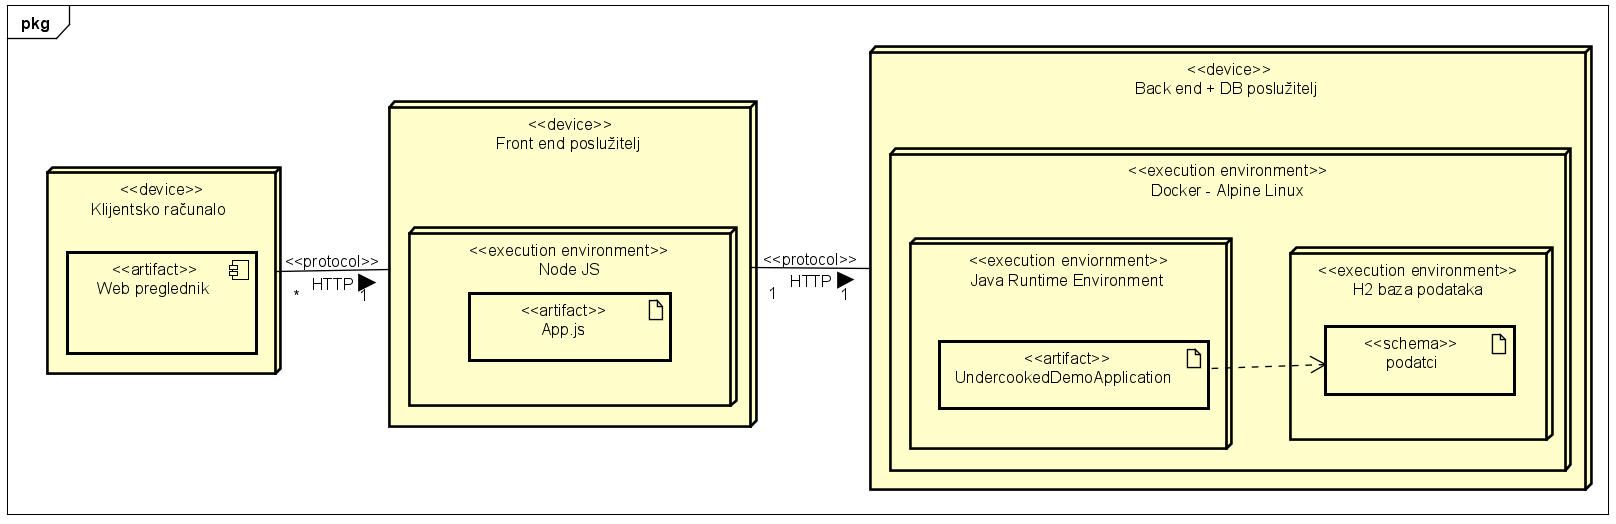
\includegraphics[scale=0.35]{slike/dijagram_razmjestaja.png} %veličina slike u odnosu na originalnu datoteku i pozicija slike
				\centering
				\caption{Dijagram razmještaja}
				\label{fig:Dijagram razmještaja}
			\end{figure}
			\eject 
		
		\section{Upute za puštanje u pogon}
		
			%\textbf{\textit{dio 2. revizije}}\\
		
			 %\textit{U ovom poglavlju potrebno je dati upute za puštanje u pogon (engl. deployment) ostvarene aplikacije. Na primjer, za web aplikacije, opisati postupak kojim se od izvornog kôda dolazi do potpuno postavljene baze podataka i poslužitelja koji odgovara na upite korisnika. Za mobilnu aplikaciju, postupak kojim se aplikacija izgradi, te postavi na neku od trgovina. Za stolnu (engl. desktop) aplikaciju, postupak kojim se aplikacija instalira na računalo. Ukoliko mobilne i stolne aplikacije komuniciraju s poslužiteljem i/ili bazom podataka, opisati i postupak njihovog postavljanja. Pri izradi uputa preporučuje se \textbf{naglasiti korake instalacije uporabom natuknica} te koristiti što je više moguće \textbf{slike ekrana} (engl. screenshots) kako bi upute bile jasne i jednostavne za slijediti.}
			
			
			 %\textit{Dovršenu aplikaciju potrebno je pokrenuti na javno dostupnom poslužitelju. Studentima se preporuča korištenje neke od sljedećih besplatnih usluga: \href{https://aws.amazon.com/}{Amazon AWS}, %\href{https://azure.microsoft.com/en-us/}{Microsoft Azure} ili \href{https://www.heroku.com/}{Heroku}. Mobilne aplikacije trebaju biti objavljene na F-Droid, Google Play ili Amazon App trgovini.}
			\subsection{Instalacija potrebne programske potpore}
			Kako bi se aplikacija ispravno pokrenula potrebno je preuzeti sljedeće programske pakete:
			\begin{itemize}
				\item \href{https://nodejs.org}{\textit{NodeJS}\footnote{https://nodejs.org}} i \href{https://www.npmjs.com}{\textit{npm}\footnote{https://www.npmjs.com}} za pokretanje front-enda
				\item \href{https://www.oracle.com/java/technologies/downloads/\#java17}{\textit{Java development kit} (Verzija 17)\footnote{https://www.oracle.com/java/technologies/downloads/\#java17}} i \href{https://maven.apache.org}{\textit{Maven}\footnote{https://maven.apache.org}} za back-end i bazu podataka.
			\end{itemize}
			\begin{figure}[H]
				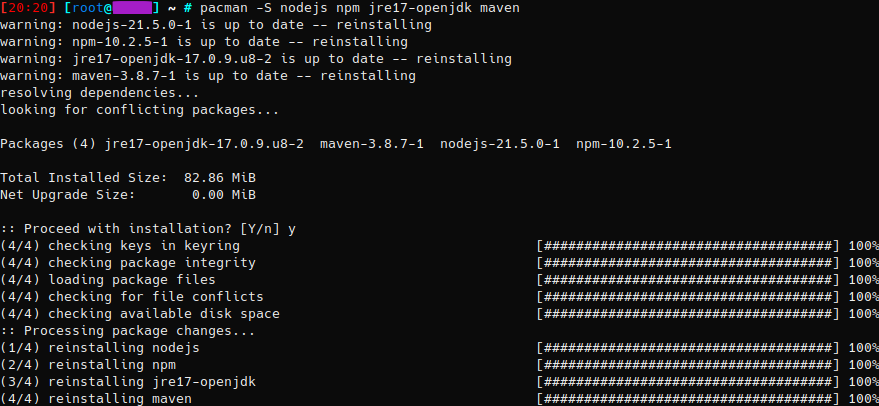
\includegraphics[scale=0.7]{slike/instalacija_1.png} %veličina slike u odnosu na originalnu datoteku i pozicija slike
				\centering
				\caption{Instalacija potrebne programske potpore na Linuxu}
				\label{fig:Instalacija potrebne programske potpore na Linuxu}
			\end{figure}
			Alternativno, back-end i baza podataka mogu se jednostavnije pokrenuti u \href{https://www.docker.com}{\textit{Docker}\footnote{https://www.docker.com}} kontejneru.
			
			Nakon instalacije navedenih programa, potrebno je klonirati repozitorij aplikacije na proizvoljnu lokaciju ili ga preuzeti kao arhivu i raspakirati.
			\begin{figure}[H]
				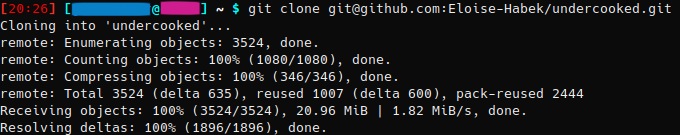
\includegraphics[scale=0.8]{slike/instalacija_2.png} %veličina slike u odnosu na originalnu datoteku i pozicija slike
				\centering
				\caption{Kloniranje repozitorija}
				\label{fig:Kloniranje repozitorija}
			\end{figure}
			\subsection{Pokretanje front-enda}
			Kako bi se pokrenuo front-end aplikacije, potrebno je pozicionirati se u direktorij \textit{IzvorniKod/undercooked-frontend} i pokrenuti \textit{npm install} kako bi se instalirale potrebne biblioteke.
			\begin{figure}[H]
				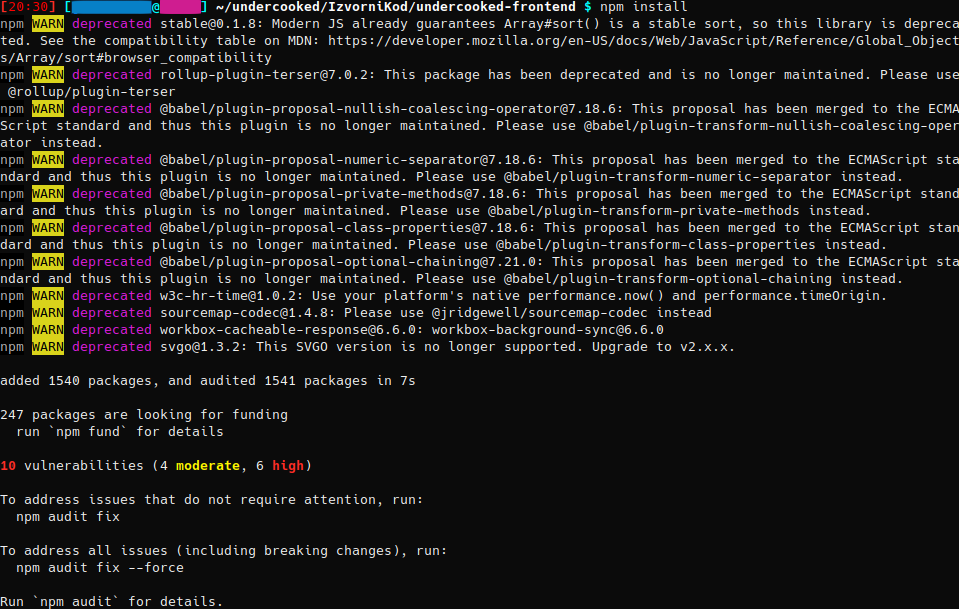
\includegraphics[scale=0.6]{slike/instalacija_3.png} %veličina slike u odnosu na originalnu datoteku i pozicija slike
				\centering
				\caption{Instalacija NodeJS biblioteka}
				\label{fig:Instalacija NodeJS biblioteka}
			\end{figure}
			Nakon toga, front-end aplikacije može se pokrenuti s \textit{npm start}. \textit{React} front-end pokreće se na vratima 3000, osim ako nije postavljena varijabla okruženja PORT.
			\begin{figure}[H]
				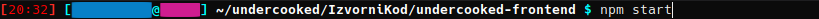
\includegraphics[scale=0.7]{slike/instalacija_4.png} %veličina slike u odnosu na originalnu datoteku i pozicija slike
				\centering
				\caption{Pokretanje front-enda}
				\label{fig:Pokretanje front-enda}
			\end{figure}
			\subsection{Pokretanje back-enda i baze podataka}
			Kako bi se pokrenuli back-end aplikacije i baza podataka, potrebno je pozicionirati se u direktorij \textit{IzvorniKod/Undercooked-Demo} i pokrenuti \textit{mvn install} čime se instalira sve što je potrebno za pokretanje back-enda i baze podataka te se gradi sama aplikacija.
			\begin{figure}[H]
				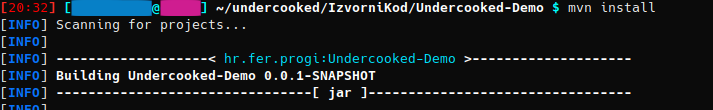
\includegraphics[scale=0.8]{slike/instalacija_5.png} %veličina slike u odnosu na originalnu datoteku i pozicija slike
				\centering
				\caption{Instalacija uz pomoć Mavena}
				\label{fig:Instalacija uz pomoć Mavena}
			\end{figure}
			Ova naredba će također pokrenuti i testove, no svi ispitni slučajevi koji koriste \textit{Selenium} će pasti jer se oslanjaju na to da back-end radi, a pokreću se prije nego što se on pokrene. Testovi se mogu izvršiti naknadno, na primjer iz IDE-a. Nakon što je izgrađena, aplikacija se može pokrenuti navigiranjem u novonastali direktorij \textit{target} i izvršavanjem naredbe \textit{java -jar Undercooked-Demo-0.0.1-SNAPSHOT.jar}. Back-end aplikacije sluša na vratima 8080, a pokretanjem back-enda pokreće se i baza podataka.
			\begin{figure}[H]
				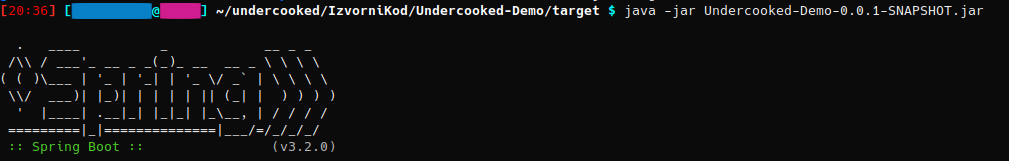
\includegraphics[scale=0.55]{slike/instalacija_6.png} %veličina slike u odnosu na originalnu datoteku i pozicija slike
				\centering
				\caption{Pokretanje back-enda i baze podataka}
				\label{fig:Pokretanje back-enda i baze podataka}
			\end{figure}
			\eject 
	\chapter{Zaključak i budući rad}
		
		\textbf{\textit{dio 2. revizije}}\\
		
		 \textit{U ovom poglavlju potrebno je napisati osvrt na vrijeme izrade projektnog zadatka, koji su tehnički izazovi prepoznati, jesu li riješeni ili kako bi mogli biti riješeni, koja su znanja stečena pri izradi projekta, koja bi znanja bila posebno potrebna za brže i kvalitetnije ostvarenje projekta i koje bi bile perspektive za nastavak rada u projektnoj grupi.}
		
		 \textit{Potrebno je točno popisati funkcionalnosti koje nisu implementirane u ostvarenoj aplikaciji.}
		
		\eject 
	\chapter*{Popis literature}
		\addcontentsline{toc}{chapter}{Popis literature}
	 	
 		\textbf{\textit{Kontinuirano osvježavanje}}
	
		\textit{Popisati sve reference i literaturu koja je pomogla pri ostvarivanju projekta.}
		
		
		\begin{enumerate}
			
			
			\item  Programsko inženjerstvo, FER ZEMRIS, \url{http://www.fer.hr/predmet/proinz}
			
			\item  I. Sommerville, "Software engineering", 8th ed, Addison Wesley, 2007.
			
			\item  T.C.Lethbridge, R.Langaniere, "Object-Oriented Software Engineering", 2nd ed. McGraw-Hill, 2005.
			
			\item  I. Marsic, Software engineering book``, Department of Electrical and Computer Engineering, Rutgers University, \url{http://www.ece.rutgers.edu/~marsic/books/SE}
			
			\item  The Unified Modeling Language, \url{https://www.uml-diagrams.org/}
			
			\item  Astah Community, \url{http://astah.net/editions/uml-new}
		\end{enumerate}
		
		 
	
	
	\begingroup
	\renewcommand*\listfigurename{Indeks slika i dijagrama}
	%\renewcommand*\listtablename{Indeks tablica}
	%\let\clearpage\relax
	\listoffigures
	%\vspace{10mm}
	%\listoftables
	\endgroup
	\addcontentsline{toc}{chapter}{Indeks slika i dijagrama}


	
	\eject 
		
	\chapter*{Dodatak: Prikaz aktivnosti grupe}
		\addcontentsline{toc}{chapter}{Dodatak: Prikaz aktivnosti grupe}
		
		\section*{Dnevnik sastajanja}
		
		\textbf{\textit{Kontinuirano osvježavanje}}\\
		
		 \textit{U ovom dijelu potrebno je redovito osvježavati dnevnik sastajanja prema predlošku.}
		
		\begin{packed_enum}
			\item  sastanak
			
			\item[] \begin{packed_item}
				\item Datum: 19. listopada 2023.
				\item Prisustvovali: E.Habek, M.Plavec, A.Dautović, L.Grubišin, A.Đurđević, M.Magat, A.Stanković
				\item Teme sastanka:
				\begin{packed_item}
					\item procjena vještina i motivacija članova tima
					\item izmijena ideja o načinu provedbe projekta
					\item upoznavanje
					\item odabir tehnologija
				\end{packed_item}
			\end{packed_item}
			
			\item  sastanak
			\item[] \begin{packed_item}
				\item Datum: 24. listopada 2023.
				\item Prisustvovali: E.Habek, M.Plavec, A.Dautović, L.Grubišin, A.Đurđević, M.Magat, A.Stanković
				\item Teme sastanka:
				\begin{packed_item}
					\item razrada projekta
					\item zajedničko iznošenje ideja za obrasce uporabe
					\item podjela posla za pisanje dokumentacije za naredni tjedan
					\item međusobno pomaganje i dijeljenje znanja o Gitu
				\end{packed_item}
			\end{packed_item}
			
			\item  sastanak
			\item[] \begin{packed_item}
				\item Datum: 31. listopada 2023.
				\item Prisustvovali: E.Habek, M.Plavec, A.Dautović, L.Grubišin, A.Đurđević, M.Magat, A.Stanković
				\item Teme sastanka:
				\begin{packed_item}
					\item 
					\item 
					\item 
					\item 
				\end{packed_item}
			\end{packed_item}
			%
			
		\end{packed_enum}
		
		\eject
		\section*{Tablica aktivnosti}
		
			\textbf{\textit{Kontinuirano osvježavanje}}\\
			
			 \textit{Napomena: Doprinose u aktivnostima treba navesti u satima po članovima grupe po aktivnosti.}

			\begin{longtblr}[
					label=none,
				]{
					vlines,hlines,
					width = \textwidth,
					colspec={X[7, l]X[1, c]X[1, c]X[1, c]X[1, c]X[1, c]X[1, c]X[1, c]}, 
					vline{1} = {1}{text=\clap{}},
					hline{1} = {1}{text=\clap{}},
					rowhead = 1,
				} 
			
				\SetCell[c=1]{c}{} & \SetCell[c=1]{c}{\rotatebox{90}{\textbf{Eloise Habek }}} & \SetCell[c=1]{c}{\rotatebox{90}{\textbf{Anabel Dautović }}} &	\SetCell[c=1]{c}{\rotatebox{90}{\textbf{Mateo Plavec }}} & \SetCell[c=1]{c}{\rotatebox{90}{\textbf{Luka Grubišin }}} &	\SetCell[c=1]{c}{\rotatebox{90}{\textbf{Alan Đurđević }}} & \SetCell[c=1]{c}{\rotatebox{90}{\textbf{Matej Magat }}} &	\SetCell[c=1]{c}{\rotatebox{90}{\textbf{Andrej Stanković }}} \\
				Upravljanje projektom 		& 1 &  &  &  &  &  & \\
				Opis projektnog zadatka 	&  &  &  & 5  &  &  & \\ 
				
				Funkcionalni zahtjevi       & 2  &  &  &  &  &  &  \\ 
				Opis pojedinih obrazaca 	&  &  &  &  &  &  &  \\ 
				Dijagram obrazaca 			&  &  &  &  &  &  &  \\ 
				Sekvencijski dijagrami 		&  &  &  &  &  &  &  \\ 
				Opis ostalih zahtjeva 		&  &  &  &  &  &  &  \\ 

				Arhitektura i dizajn sustava	 &  &  &  &  &  &  &  \\ 
				Baza podataka				&  &  &  &  &  &  &   \\ 
				Dijagram razreda 			&  &  &  &  &  &  &   \\ 
				Dijagram stanja				&  &  &  &  &  &  &  \\ 
				Dijagram aktivnosti 		&  &  &  &  &  &  &  \\ 
				Dijagram komponenti			&  &  &  &  &  &  &  \\ 
				Korištene tehnologije i alati 		&  &  &  &  &  &  &  \\ 
				Ispitivanje programskog rješenja 	&  &  &  &  &  &  &  \\ 
				Dijagram razmještaja			&  &  &  &  &  &  &  \\ 
				Upute za puštanje u pogon 		&  &  &  &  &  &  &  \\  
				Dnevnik sastajanja 			& 1 &  &  &  &  &  &  \\ 
				Zaključak i budući rad 		&  &  &  &  &  &  &  \\  
				Popis literature 			&  &  &  &  &  &  &  \\  
				&  &  &  &  &  &  &  \\ \hline 
				\textit{Postavljanje programske potpore} 			&  &  & 2 & 1  &  &  &  \\
				\textit{GitHub admin} 			&  &  & 3 &  &  &  &  \\
				\textit{Dodatne stavke kako ste podijelili izradu aplikacije} 			&  &  &  &  &  &  &  \\ 
				\textit{npr. izrada početne stranice} 				&  &  &  &  &  &  &  \\  
				\textit{izrada baze podataka} 		 			&  &  &  &  &  &  & \\  
				\textit{spajanje s bazom podataka} 							&  &  &  &  &  &  &  \\ 
				\textit{back end} 							&  &  &  &  &  &  &  \\  
				 							&  &  &  &  &  &  &\\ 
			\end{longtblr}
					
					
		\eject
		\section*{Dijagrami pregleda promjena}
		
		\textbf{\textit{dio 2. revizije}}\\
		
		\textit{Prenijeti dijagram pregleda promjena nad datotekama projekta. Potrebno je na kraju projekta generirane grafove s gitlaba prenijeti u ovo poglavlje dokumentacije. Dijagrami za vlastiti projekt se mogu preuzeti s gitlab.com stranice, u izborniku Repository, pritiskom na stavku Contributors.}
		
	


\end{document} %naredbe i tekst nakon ove naredbe ne ulaze u izgrađen dokument 


